\documentclass[runningheads]{llncs}

\usepackage{amsmath,amssymb}
\usepackage{array,booktabs,float,graphicx,listings,multirow,xcolor,tikz,url}
\usepackage{longtable,capt-of,needspace,xr}
\usetikzlibrary{arrows.meta,backgrounds,fit}
\emergencystretch=1.5em

\definecolor{vanilla}{RGB}{75,105,145}
\definecolor{flexible}{RGB}{0,125,120}
\definecolor{slotblue}{RGB}{20,85,155}
\definecolor{slotorange}{RGB}{180,80,10}
\newcommand{\Tool}{\textsc{acgn}}
\newcommand{\CanDis}{\textsc{CanDis}}
\newcommand{\Seq}{\texttt{Seq}}
\newcommand{\Bag}{\texttt{Bag}}
\newcommand{\Set}{\texttt{Set}}
\newcommand{\TEmb}{\operatorname{TEmb}}
\newcommand{\TRen}{\operatorname{TRen}}
\newcommand{\EqCert}{\operatorname{EqCert}}
\newcommand{\Rep}{\operatorname{Rep}}

\newcommand{\Fix}[1]{\textcolor{blue}{#1}}

% Machine-readable paper--Lean correspondence tag.  The second argument is
% the frozen fully qualified Lean declaration name; tags are visually silent.
\providecommand{\leanref}[2]{}


\title{Typed Flexible-Arity Slotted E-Graphs:\\
Soundness and an Alloy Case Study}
\titlerunning{Typed Flexible-Arity Slotted E-Graphs}
\author{Anonymous Author(s)}
\institute{}

\ifdefined\FullDraft\else
\externaldocument{supplement}
\fi
\begin{document}
\maketitle
\begin{abstract}
Algebraic normalization and sharing of open expressions interact whenever an
associative, commutative, or idempotent operator combines subterms whose free
variables come from outer binders. We present typed flexible-arity slotted
e-graphs, which compose sequence, bag, and set ports—whose sibling equations
and recursive flattening licenses are certified separately—with explicit typed
maps for open-term interfaces. Canonicalization separates an expression's
effective-support kernel from its placement in the caller context. Over the
abstract formal model, we prove four results formalized in Lean: complete
finite quotient presentations yield exact canonical shapes; structural
realization and compatible shape collisions preserve source equations; and
graph updates preserving a local coherence invariant give sound judgments
between finite unfoldings.

We evaluate \CanDis{} in an Alloy case study across 66,080 student--oracle
specification files (61,598 eligible distinct-AST comparisons and 4,482
AST-identical paired rows) and a 5,500-pair controlled transformation suite.
Both rewrite paths found 4,499 structural zeros among the correct
distinct-AST pairs, retaining every one of the 2,228 original slotted
zeros. Neither path assigned zero to a labeled incorrect pair. Five rule
families tested under the original Alloy command recognized 259 additional
correct pairs. Across 181 correct-reference pools, 4,496 unique raw ASTs
yielded 2,016 structural forms and 1,942 fixed-command components. On a separate controlled suite,
CanDis recognized 5,500 of 5,500 pairs, compared with
3,628 for the De Bruijn baseline.
\keywords{E-graphs \and Binding \and AC rewriting \and Alloy \and
Canonical intermediate representations}
\end{abstract}
\section{Introduction}

Relational specification languages such as Alloy~\cite{alloy,kodkod} let users
express the same constraint in many syntactically distinct ways. Consider two
Alloy predicates describing the same social-media visibility rule—a photo seen
by a user must either come from a followed user or be an advertisement:
\begin{center}
\footnotesize
\begin{tabular}{@{}p{0.47\linewidth}@{\hspace{1.2em}}p{0.47\linewidth}@{}}
\begin{minipage}[t]{\linewidth}\ttfamily
pred left \{\\
\hspace*{1em}all u: User, p: Photo |\\
\hspace*{2em}p in u.sees implies\\
\hspace*{3em}(p not in Ad) implies\\
\hspace*{4em}p in u.follows.posts\\
\hspace*{4em}or p in Ad\\
\}
\end{minipage}
&
\begin{minipage}[t]{\linewidth}\ttfamily
pred right \{\\
\hspace*{1em}all photo: Photo, user: User |\\
\hspace*{2em}photo in user.sees implies\\
\hspace*{3em}photo in Ad or\\
\hspace*{3em}photo in user.follows.posts\\
\}
\end{minipage}
\end{tabular}
\end{center}
To a raw abstract syntax tree (AST) comparator, \texttt{left} and \texttt{right}
differ at almost every node: nested implications versus a single implication, a
repeated \texttt{p in Ad} test, reversed disjunction operands, renamed bound
variables (\texttt{u, p} vs.\ \texttt{user, photo}), and swapped declarations
(\texttt{User, Photo} vs.\ \texttt{Photo, User}). Yet rewriting implications
into disjunctions exposes three flat operands over the same two-variable body,
allowing idempotence and commutativity to collapse \texttt{left} and
\texttt{right} to the same canonical shape once their typed variables are
aligned.

This example illustrates a general coupling in e-graphs~\cite{ogEgraphs1,egraphsOG,egg,eqsat,eqsat-lmcs}
between \emph{algebraic normalization} and \emph{open-term sharing}. Suppose an
open expression is the conjunction
\[
 P(x,y)\land P(y,x),
\]
such as \texttt{u in v.follows and v in u.follows} inside a quantifier over
\texttt{u, v: User}. Associativity and commutativity suggest storing
conjunction as a flat container, and idempotence suggests a set. Yet
\texttt{u in v.follows} and \texttt{v in u.follows} share the same open-term
shape while assigning different caller variables to its argument positions. They
can collapse into one set element only if the graph has proved $P(x,y)=P(y,x)$;
otherwise, equating them would falsely turn an asymmetric relation into a
symmetric one. Similarly, when simplification eliminates a variable (for
instance, removing an unused binder), the canonical shape should contract to the
remaining \emph{effective support} while preserving its embedding into the
original caller context.

We compose flexible-arity sequence, bag, and set ports with typed slotted
interfaces. An invocation $m*a$ pairs an e-class $a$ with an injective,
type-preserving map $m$ into the caller context, while recorded class symmetries
justify specific slot rearrangements. Canonicalization extracts a kernel over
its effective support, normalizes local invocation and binder-block orbits
before deduplicating bags and sets, and selects a least representative modulo
typed renaming. Types partition the renaming search space by variable sort, and
separate licenses govern sibling laws and recursive flattening.

Our formal argument establishes two guarantees over this abstract model:
canonical shapes identify exactly the declared structural equivalence classes
over effective supports (Theorem~\ref{thm:shape-exactness}), and equality
judgments extracted from finite unfoldings hold in every model of the source
equational theory (Propositions~\ref{thm:structural-soundness}
and~\ref{thm:collision-soundness}, Theorem~\ref{thm:semantic-sound}). All four
proofs appear in the main text, and Appendix~\ref{app:formal-details} records the
exact mapping to our Lean~4.33.0 formalization.

In Alloy, our canonical distance pipeline \CanDis{} distinguishes
\emph{canonical equality} from \emph{repair distance}. For \texttt{left} and
\texttt{right} above, both forms have distance zero under the implemented
rewrite theory. If a student instead writes \texttt{photo in user.sees implies
photo in user.follows.posts}—omitting \texttt{or photo in Ad}—canonical
equality fails because the predicate is genuinely overconstrained, and
\CanDis{} computes a positive structural edit distance over its normalized
repair projection to locate nearby correct solutions.

In a supervised run over 66,080 Alloy4Fun files, both \CanDis{} paths
recognized 5,137 of 19,212 correct distinct-AST student--oracle
pairs. They retained all 2,228 original Slotted zeros, recognized
2,909 additional pairs, and assigned positive distances to all
42,386 incorrect pairs. Across 181 invariant pools, the
4,496 distinct correct reference ASTs reduced to 1,816 structural
forms. Adding equalities verified under the exercise commands connected these
forms into 1,743 components (Section~\ref{sec:scoped-pools}).
For incorrect submissions, the mean distance to the nearest correct reference
was 12.267 raw-AST edits or 11.478 edits under \CanDis{}.

\section{Background and Scope}
\label{sec:background}

\paragraph{E-graphs and equality saturation.}
An \emph{e-node} stores an operator and references to child \emph{e-classes},
where each e-class groups expressions already known to be equal~\cite{ogEgraphs1,egraphsOG,egg}.
For example, given $a\times 2=a+a$ and singleton classes $c_a=\{a\}$ and
$c_2=\{2\}$, a single class $c=\{\times(c_a,c_2),\;+(c_a,c_a)\}$ shares both
forms, and a parent $g(c)$ compactly represents both $g(a\times 2)$ and
$g(a+a)$ (Figure~\ref{fig:typed-slotted-egraphs}(a)).
% Preamble: \usepackage{graphicx,amsmath,amssymb}
% Place typed-slotted-egraphs.pdf beside the main LaTeX source.
\begin{figure}[t]
  \centering
  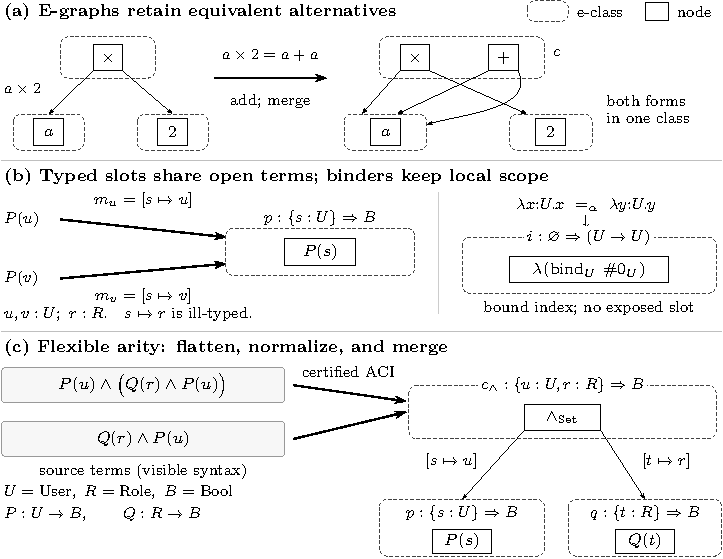
\includegraphics[width=\linewidth]{figures/typed-slotted-egraph-figure.pdf}
  \caption{E-graphs, typed slots, and flexible arity.
  (a) Rewriting retains equivalent alternatives.
  (b) Typed maps share shapes without equating distinct free invocations;
  bound indices stay local.
  (c) Certified associativity flattens visible syntax; the Set quotient removes
  order and duplicates. Dashed boxes are e-classes; solid inner boxes are e-nodes.}
  \label{fig:typed-slotted-egraphs}
\end{figure}

Propagating child merges to parents is \emph{congruence}. After union--find
merges classes, \emph{rebuilding} restores hash-cons invariants and propagates
new parent congruences. Equality saturation alternates rewriting and rebuilding
until saturation or a resource bound, and extraction picks a term under a cost
model. Our focus is how e-node keys and equality certificates combine algebraic
containers with typed open-term interfaces.

\paragraph{Algebraic structure.}
Associativity, commutativity, and idempotence play distinct roles. For
conjunction, associativity flattens nested binary nodes, commutativity ignores
operand order, and idempotence drops duplicates. Sequences preserve order and
multiplicity, bags preserve multiplicity only, and sets preserve neither. Flat
bags and sets avoid combinatorial blowup in AC rewriting~\cite{conchon2012canonized,kapur2021ModularAC}:
over $n$ distinct generators, complete binary AC closure creates $2^n-1$
nonempty subproduct classes and $3^n+1-2^{n+1}$ ordered binary nodes
(Appendix~\ref{app:formal-details}). Relational fixpoint engines such as
egglog~\cite{egglog,egglog_software} and E-graphs Modulo
Theories~\cite{zucker2025omeletsneedonionsegraphs} connect e-graphs with
canonical algebraic values; here we study how container quotients interact with
typed variable bindings.

\paragraph{Binding and typed slots.}
Renaming bound variables yields $\alpha$-equivalence, as in
$\forall x{:}T.\,P(x)$ and $\forall y{:}T.\,P(y)$
(Figure~\ref{fig:typed-slotted-egraphs}(b)). When sharing an open body $P(x)$
across contexts, each occurrence must record which caller variable supplies $x$.
Slotted e-graphs~\cite{slottedEGraphs} attach a finite slot interface $S_a$ to
each class $a$ and write an occurrence as $m*a$, where $m$ maps $S_a$ into the
caller context. In our typed setting, a \texttt{User} slot maps only to a
\texttt{User} coordinate and a \texttt{Photo} slot only to a \texttt{Photo}
coordinate, while distinct variables of the same sort remain distinct slots.
Related approaches represent open terms functionally~\cite{zucker2026lifting} or
via hierarchical hypergraphs~\cite{egBindings}. We use de Bruijn
indices~\cite{deBruijn,maziarz2021HashingAlpha} for local bound positions and
typed slots for free positions. A binder-block descriptor records types,
domains, multiplicities, disjointness, and dependencies so that only
semantically justified block permutations enter the structural relation.

\paragraph{Alloy and bounded checking.}
Alloy~\cite{alloy,kodkod} models relational structures and temporal formulas
over signatures and fields. In the social-media model used in our running
example (Figure~\ref{fig:alloy-certificate-example}), \texttt{User} and
\texttt{Photo} are signatures, \texttt{Ad} extends \texttt{Photo}, and fields
such as \texttt{follows: set User} and \texttt{sees: set Photo} declare binary
relations. Relational join (\texttt{u.follows.posts}) composes relations,
membership (\texttt{p in u.sees}) tests containment, and quantifiers
(\texttt{all u: User | ...}) range over typed sets. The Alloy Analyzer checks
formulas within finite object scopes and trace bounds. In our Alloy4Fun
corpus~\cite{alloy4funDataset2023,alloy4fun,novice}, student submissions are
labeled relative to an oracle: \texttt{CORRECT}, overconstrained (excluding
valid instances), underconstrained (admitting invalid instances), or both.

\paragraph{Formal vs.\ empirical scope.}
Throughout the paper, we separate three kinds of claims:
(1)~\emph{formal-model theorems} proved in Lean~4.33.0 about abstract typed
slotted presentations, realizers, and certificate-preserving graph traces;
(2)~\emph{implementation checks} executed on the Java system (in-process strict
transition invariants, standalone certificate-verifier tests, bounded Alloy
counterexample searches, and native-operation replay audits); and
(3)~\emph{empirical observations} measured on natural, controlled, and synthetic
workloads. Observed agreement between two Java implementations is an empirical
check on those runs, not a universal equivalence proof, and end-to-end formal
refinement from Alloy source through the Java parser to Lean remains open.

\section{Typed Flexible-Arity Slotted E-Graphs}
\label{sec:formalism}

We fix a typed source signature and a choice of source equational laws. The
representation separates three responsibilities: typed maps describe how an open
expression is placed into a caller, ports describe the algebraic structure of
an operator's children, and graph records track equations already proved.

\paragraph{Two source equalities.}
If both operands are unary relations, domain and range restriction select
exactly the atoms in their intersection. This does not replace restriction
of a binary relation: that operation selects tuples by one column.
For a fixed domain $D$, $\forall x\in D.\,\Box P(x)$ and
$\Box(\forall x\in D.\,P(x))$ both require $P(x)$ for every atom in $D$
at every future instant. An empty $D$ is allowed. If $D$ can grow or
shrink, the two formulas inspect different bindings; the rewrite is then
not justified. The appendix gives the Lean statements and negative controls.

\subsection{Contexts, invocations, and ports}

A \emph{typed context} $\Gamma$ is a finite collection of distinct slots, each
carrying a type. A \emph{typed embedding} is an injective, type-preserving map;
a \emph{typed renaming} is an embedding with a typed inverse:
\[
 \TEmb(S,T)=\{m:S\hookrightarrow T\mid
                    \operatorname{ty}(m(x))=\operatorname{ty}(x)\},
\]
and $\TRen(S,T)$ denotes the typed renamings. Identities and composites are
embeddings, and renamings are closed under inverse and composition. Fixing a
linear order on types defines a canonical context $\operatorname{Can}(S)$: list
types in order and index the slots of each type from $0$. This preserves the
slot count of each type without retaining original variable names.

An e-class $a$ has interface $S_a$ and output type $\tau_a$. An
\emph{invocation} of $a$ in caller $\Gamma$ is $m*a$, where
$m\in\TEmb(S_a,\Gamma)$; its type is $\tau_a$. We abbreviate
$\operatorname{id}_{S_a}*a$ by $a$. The map is part of the occurrence: two
invocations of the same class can supply different caller variables.

Each type-instantiated operator $f_\theta$ declares input \emph{ports} using
containers $\Seq$, $\Bag$, or $\Set$ (sequences, multisets, or sets) paired
with a nonempty set $J\subseteq\mathbb N$ of legal arities ($K^+$ for positive
arities, $K^{=k}$ for arity $k$):
\[
 \kappa ::= \texttt{One}(\tau)\mid K^J(\kappa)
 \mid\texttt{Bind}(\tau,\kappa)\mid\texttt{BindBlock}(\beta,\kappa),
 \qquad K\in\{\Seq,\Bag,\Set\}.
\]
Checked syntax retains occurrence vectors even for bag and set ports so
provenance can track duplicate removal and reordering; normalization then
computes the sequence, multiset, or set key. A typed node has the form
\[
 n=f_\theta(q_1,\ldots,q_r),\qquad
 q_i\in\operatorname{Port}_\Gamma(\kappa_i),\qquad
 \operatorname{out}(n)=\tau_{f_\theta}.
\]
Port atoms are free slots, typed de Bruijn bound indices, or invocations.
Binders extend the local de Bruijn scope. A binder-block descriptor $\beta$
records types, domains, multiplicities, disjointness, and dependencies,
together with an admitted subgroup $\operatorname{Aut}(\beta)$ of typed bound
permutations whose elements preserve meaning under the descriptor's conditions.

\paragraph{Licensed container laws.}
A $\Seq$ port requires no sibling equation, $\Bag$ requires commutativity, and
$\Set$ requires commutativity and idempotence. Recursive flattening is licensed
separately: it applies only to a sole root container with matching element and
result types, requires associativity for that exact operator instance, and
requires arity closure:
\begin{align*}
 k\in J,\ 1\le j\le k &\implies j\in J &&(\text{for }\Set),\\
 k,l\in J,\ k>0 &\implies k+l-1\in J &&(\text{for flat}).
\end{align*}
If a flat port admits zero operands, the source theory must also supply a unit.
These laws must be justified by the source theory for the exact operator
instance: conjunction uses a flat $\Set$, equality uses a commutative binary
port without flattening, and integer addition uses a $\Bag$ whose flattening
depends on whether arithmetic is modular or overflow-checked.

\paragraph{Renaming and support.}
The free support $\operatorname{slots}(v)$ collects the free slots in an
expression: a free slot contributes itself, $m*a$ contributes $\operatorname{im}(m)$,
bound indices contribute nothing, and composites take the union of their
children. Any embedding $e\in\TEmb(\Gamma,\Gamma')$ acts componentwise, fixes
bound indices, and maps $m*a$ to $(e\circ m)*a$. By structural induction,
this action preserves schemas and output types and satisfies
\begin{equation}
 \operatorname{slots}(e\cdot v)=e[\operatorname{slots}(v)].
 \label{eq:support-action}
\end{equation}

\subsection{A worked example: sharing without losing variables}
\label{sec:worked-example}

Let class $a$ represent the Alloy relation test $x\in y.\mathsf{follows}$ over
$S_a=\{s:\mathsf{User},\,t:\mathsf{User}\}$, and let the caller have
$x,y:\mathsf{User}$. The two maps
$m(s)=x, m(t)=y$ and $m'(s)=y, m'(t)=x$ give invocations
$m*a=(x\in y.\mathsf{follows})$ and $m'*a=(y\in x.\mathsf{follows})$. Inside
a conjunction $\Set$ port $\{m*a,m'*a\}$, both invocations share class $a$ but
remain distinct elements because $m\neq m'$. If the graph establishes
$s\in t.\mathsf{follows}\iff t\in s.\mathsf{follows}$ and records the swap
$\pi(s)=t, \pi(t)=s$ as a symmetry of $a$, then $m'=m\circ\pi$ puts both
invocations in one local orbit. Normalizing that orbit before forming the set
collapses $\{m*a,m'*a\}$ to one element; under a $\Bag$, both multiplicities
remain, giving multiplicity~2; under a $\Seq$, both positions remain.

A caller renaming acts globally on an entire kernel—renaming $(x,y)$ to
$(u,v)$ preserves the relationship between $m$ and $m'$—whereas class
symmetries act per invocation and binder-block permutations act only within a
quantifier or comprehension block whose descriptor conditions admit them.

\subsection{Graph structure and effective support}

A finite graph stores class interfaces, typed node cases, parent links, and
recorded interface symmetries. A parent link $a\xrightarrow{p}b$ carries
$p\in\TEmb(S_b,S_a)$ between classes of equal output type. The parent forest has
decreasing depths, so leader lookup terminates at a root $\ell$ with composite
embedding $p_a\in\TEmb(S_\ell,S_a)$, sending $m*a$ to $\widehat m*\ell$ where
$\widehat m=m\circ p_a$. Because $p_a$ need not be surjective,
\begin{equation}
 \operatorname{im}(m\circ p_a)\subseteq\operatorname{im}(m),
 \label{eq:find-support}
\end{equation}
so leader normalization can contract the exposed support.

Each leader $\ell$ records a group $G_\ell$ of justified typed symmetries. Two
leader invocations align under a caller renaming $\rho\in\TRen(\Gamma,\Gamma')$
when their leaders coincide and there exists $\pi\in G_\ell$ such that
\begin{equation}
 \rho\circ\widehat m=\widehat m'\circ\pi.
 \label{eq:invocation-alignment}
\end{equation}
The structural equivalence relation compares sequences pointwise, bags by an
occurrence bijection, sets by mutual forward and backward matching, unary
binders by preserving the bound index, and binder blocks via admitted
descriptor permutations, closed under reflexivity, symmetry, and transitivity.
By composing~\eqref{eq:invocation-alignment} with inverses, caller renamings
transport alignments via conjugation and leader symmetries preserve image
supports.

\subsection{Canonical shapes}
\label{sec:algorithm}

Canonicalization first follows parent links and applies licensed local
simplifications to extract a \emph{kernel} $K_n$ over its effective support
$\Delta_n\subseteq\Gamma_n$, retaining the support inclusion
$\iota_n\in\TEmb(\Delta_n,\Gamma_n)$ and finite provenance between $n$ and
$\iota_n\cdot K_n$. Within $K_n$, child and binder orbits are normalized before
aggregating bags or deduplicating sets, and a least representative is chosen
under free-slot renaming.

To state exactness abstractly, a \emph{finite quotient presentation} fixes a
linearly ordered carrier $X$, a local structural generator whose generated
equivalence $\sim$ is decidable, a finite list enumerating every candidate in
$X$ (\emph{carrier completeness}), and invariants asserting that each generator
step preserves support, schema, leaf types, and output type. Define
$Q(x)=\min\{y\in X\mid y\sim x\}$. An \emph{effective-support canonicalizer}
additionally maps each node $n$ to an effective kernel $K_n$ over effective
context $\Delta_n$, an inclusion $\iota_n\in\TEmb(\Delta_n,\Gamma_n)$, a
constructive witness selector for $\sim$, and kernel preservation of support,
schema, leaf types, and output type, such that $K_n$ and $K_{n'}$ are related
by the presentation equivalence if and only if a typed renaming
$\rho\in\TRen(\Delta_n,\Delta_{n'})$ carries a structural derivation
$K_n\Rightarrow_\rho K_{n'}$. Put $\operatorname{Shape}(n)=Q(K_n)$.

\begin{theorem}[Effective-support canonical-shape exactness]
\label{thm:shape-exactness}
Under a finite quotient presentation, $Q(x)\sim x$, $Q(Q(x))=Q(x)$,
$Q(x)=Q(y)\iff x\sim y$, and $Q$ preserves support, schema, leaf types, and
output type. Consequently, for any effective-support canonicalizer as above and
nodes $n,n'$,
\[
 \operatorname{Shape}(n)=\operatorname{Shape}(n')
 \quad\Longleftrightarrow\quad
 \exists\rho\in\TRen(\Delta_n,\Delta_{n'}).\ K_n\Rightarrow_\rho K_{n'},
\]
and either side implies $\operatorname{out}(n)=\operatorname{out}(n')$.
Moreover, the constructed canonical record supplies a witness
$\sigma_n\in\TRen(C_n,\Delta_n)$ (where $C_n=\operatorname{Can}(\Delta_n)$)
and ambient transport $\omega_n=\iota_n\circ\sigma_n\in\TEmb(C_n,\Gamma_n)$.
\end{theorem}
\begin{proof}
For every $x\in X$, the finite orbit $\{y\in X\mid y\sim x\}$ is nonempty because
$x\sim x$, so its minimum $Q(x)$ exists and satisfies $Q(x)\sim x$. If $x\sim y$,
symmetry and transitivity identify their orbits, giving $Q(x)=Q(y)$;
conversely, $Q(x)=Q(y)$ implies $x\sim Q(x)=Q(y)\sim y$. Setting $y=Q(x)$ yields
idempotence. Induction on the reflexive--symmetric--transitive closure lifts
support, schema, leaf-type, and output-type invariance from each generator to
$\sim$, and hence to $Q(x)\sim x$.

Applying this exactness to $K_n$ and $K_{n'}$ and composing with the
presentation-to-derivation equivalence yields
\[
 \operatorname{Shape}(n)=\operatorname{Shape}(n')
 \iff
 \exists\rho\in\TRen(\Delta_n,\Delta_{n'}).\ K_n\Rightarrow_\rho K_{n'}.
\]
Either side puts $K_n$ and $K_{n'}$ in the same $\sim$-orbit, preserving
$\operatorname{out}(K_n)=\operatorname{out}(n)$. Because $Q(K_n)\sim K_n$, the
constructive selector yields a witness $\sigma_n\in\TRen(C_n,\Delta_n)$ and
composing with $\iota_n$ yields $\omega_n=\iota_n\circ\sigma_n$.\qed
\end{proof}

\paragraph{Why carrier completeness and effective support matter.}
If enumeration stops early under a heuristic budget instead of satisfying
carrier completeness, equal shapes still witness equivalence ($\Rightarrow$),
but two structurally equivalent expressions need not select the same minimum
($\Leftarrow$). For example, consider the open Alloy body \texttt{p in Ad} in contexts
$(u\!:\!\mathsf{User},p\!:\!\mathsf{Photo})$ and $(p\!:\!\mathsf{Photo})$.
In each context the body reads only $p$. Its effective support therefore
contains one photo slot, so the identity on that slot matches the two shapes.

\subsection{Building canonical records and search cost}
\label{sec:canonicalization-procedure}

A canonical record $(K_n,p_n,\sigma_n,\iota_n)$ stores the kernel $K_n$, least
shape $p_n=\operatorname{Shape}(n)$, witness $\sigma_n:C_n\cong\Delta_n$,
inclusion $\iota_n:\Delta_n\hookrightarrow\Gamma_n$, and extraction/normalization
provenance. Construction proceeds in four steps:
(1)~follow leaders, apply licensed local rules, and flatten visible matching
operators;
(2)~compute the effective support $\Delta_n$, forming $K_n$ and $\iota_n$;
(3)~for each typed bijection $\sigma\in\TRen(C_n,\Delta_n)$, apply
$\sigma^{-1}$ to $K_n$, normalize local invocation and binder orbits, and
aggregate bags or deduplicate sets;
(4)~select the least resulting shape $p_n$ and retain $\sigma_n$ and its
derivation.
Only $p_n$ acts as the collision key; the remaining fields place the shape in
$\Gamma_n$.

When a child merge or new symmetry triggers \emph{rebuilding}, affected parent
records are recomputed and colliding keys are checked against output types and
maps. Crucially, the exact enumeration in step~(3) searches
$\prod_\tau|\Delta_{n,\tau}|!$ typed bijections, where $\Delta_{n,\tau}$ is
the fibre of slots of type $\tau$. Slots of distinct types never mix in the
permutation search, whereas $N$ slots of a single type retain the full $N!$
search space—a scaling behavior we measure directly in Section~\ref{sec:eval-synthetic}.

\begin{figure}[t]
\centering
\scriptsize
\setlength{\fboxsep}{4pt}

\fbox{%
\begin{minipage}{0.94\linewidth}
\textbf{Model context}\par
\ttfamily
sig User \{ follows: set User, sees: set Photo, posts: set Photo \}\\
sig Photo \{ date: one Day \}\hspace{1.8em}%
sig Ad extends Photo \{\}\hspace{1.8em}sig Day \{\}
\end{minipage}%
}

\vspace{4pt}

\begin{minipage}[t]{0.47\linewidth}
\raggedright
\textbf{LEFT}\par
\ttfamily
pred left \{\\
\hspace*{1em}all u: User, p: Photo |\\
\hspace*{2em}p in u.sees implies\\
\hspace*{3em}(p not in Ad) implies\\
\hspace*{4em}p in u.follows.posts or p in Ad\\
\}
\end{minipage}
\hfill
\begin{minipage}[t]{0.47\linewidth}
\raggedright
\textbf{RIGHT}\par
\ttfamily
pred right \{\\
\hspace*{1em}all photo: Photo, user: User |\\
\hspace*{2em}photo in user.sees implies\\
\hspace*{3em}photo in Ad or\\
\hspace*{3em}photo in user.follows.posts\\
\}
\end{minipage}

\vspace{4pt}

\begin{minipage}{0.95\linewidth}
Let
\(A(x,y)\equiv y\in x.\mathsf{sees}\),
\(B(x,y)\equiv y\in x.\mathsf{follows}.\mathsf{posts}\), and
\(C(y)\equiv y\in\mathsf{Ad}\).
Under the canonical context
\(\Gamma_Q=\{q_0:\mathsf{User},\,q_1:\mathsf{Photo}\}\):
\[
\begin{aligned}
\mathsf{left}
&\stackrel{\mathrm{Imp},\,\alpha_{\Gamma_Q}}{\Longrightarrow}
  \neg A(q_0,q_1)\lor C(q_1)\lor B(q_0,q_1)\lor C(q_1)
\stackrel{\mathrm{ACI}_{\lor}}{\Longrightarrow} Q,
\\
\mathsf{right}
&\stackrel{\mathrm{Imp},\,\alpha_{\Gamma_Q},\,\pi_{\mathrm{bind}}}{\Longrightarrow}
  \neg A(q_0,q_1)\lor C(q_1)\lor B(q_0,q_1)
\stackrel{\mathrm{ACI}_{\lor}}{\Longrightarrow} Q.
\end{aligned}
\]
\end{minipage}

\vspace{2pt}

\fbox{%
\begin{minipage}{0.94\linewidth}
{\centering\textbf{Shared canonical form $Q$ (distance $0$ between \texttt{left} and \texttt{right})}\par}
\ttfamily
all \_q0: User, \_q1: Photo |\\
\hspace*{1em}\_q1 not in \_q0.sees or \_q1 in Ad or \_q1 in \_q0.follows.posts
\end{minipage}%
}

\vspace{3pt}

\begin{minipage}{0.95\linewidth}
\textbf{Inequivalent variant (repair distance $>0$):}\quad
{\ttfamily pred bug \{ all user: User, photo: Photo | photo in user.sees implies photo in user.follows.posts \}}
omits {\ttfamily photo in Ad}. Canonical equality fails ($d>0$), and repair
distance measures structural edits between the normalized projection of
\texttt{bug} and $Q$.
\end{minipage}

\caption{Running Alloy example. Implication elimination exposes flat
disjunctions, typed renaming and independent binder permutation align
\texttt{User} and \texttt{Photo} coordinates to $\Gamma_Q$, and
$\Set$-port normalization drops order and the duplicate \texttt{p in Ad}.}
\label{fig:alloy-certificate-example}
\end{figure}


Figure~\ref{fig:alloy-certificate-example} returns to our opening Alloy
example. Implication elimination exposes flat disjunctions, typed renaming and
independent binder permutation align the \texttt{User} and \texttt{Photo}
slots into $\Gamma_Q$, and $\Set$-port normalization removes operand order and
the duplicate \texttt{p in Ad}, yielding distance~0 between \texttt{left} and
\texttt{right} under the implemented rewrite theory. By contrast, \texttt{bug}
omits \texttt{photo in Ad}, so canonical equality fails ($d>0$), and repair
distance measures edits between its normalized repair projection and $Q$.

\section{An Algebraic Soundness Argument}
\label{sec:metatheory}

We now connect structural derivations, shape collisions, and graph updates to
the typed source equational theory $\mathcal T$, whose derivations
$\mathcal T\vdash_\Gamma s=t$ are generated by primitive laws, forward
congruence, reflexivity, symmetry, transitivity, and transport along embeddings
$e\in\TEmb(\Gamma,\Gamma')$. In every typed model $\mathfrak M$ validating the
primitive laws and congruence rules, environment restriction satisfies
$\operatorname{eval}_{\mathfrak M}(e\cdot t,\eta')
=\operatorname{eval}_{\mathfrak M}(t,\eta'\circ e)$, so every derivable
certificate holds semantically in $\mathfrak M$.

\subsection{From structural derivations to source equations}

A \emph{typed structural realizer} $R$ interprets port atoms, containers,
unary binders, binder blocks, and nodes as source terms and commutes with every
embedding $e$. Constructor laws supply one-step equational certificates for
$\Seq$ (positional bijection), $\Bag$ (occurrence bijection), $\Set$ (mutual
forward and backward matching maps), unary binders (scope extension),
descriptor-admissible binder-block permutations, and outer nodes, while leaf
steps carry individual equational certificates.

\begin{proposition}[Structural realization and congruence soundness]
\label{thm:structural-soundness}
Given a typed structural realizer $R$ commuting with embeddings, licensed
constructor congruence laws, and per-leaf equational certificates, every direct
structural derivation from $v$ to $v'$ under $e\in\TEmb(\Gamma,\Gamma')$ yields
\[
 \mathcal T\vdash_{\Gamma'} e\cdot R(v)=R(v'),
 \qquad
 \operatorname{eval}_{\mathfrak M}(e\cdot R(v),\eta)
 =\operatorname{eval}_{\mathfrak M}(R(v'),\eta)
\]
in every typed model $\mathfrak M$ and environment $\eta$. The same holds for
the indexed reflexive--symmetric--transitive closure under typed renamings
$\rho\in\TRen(\Gamma,\Gamma')$, including descriptor-admissible binder-block
permutations.
\end{proposition}
\begin{proof}
Structural induction gives naturality $R(e\cdot v)=e\cdot R(v)$ from the
supplied constructor commutation equations. Induction on the direct structural
derivation then constructs the equational certificate: leaf steps use their
supplied certificates; $\Seq$, $\Bag$, $\Set$, unary-binder, and binder-block
cases apply the corresponding licensed constructor law to the inductive child
certificates; and node steps apply node congruence.

For the closure indexed by renamings, reflexivity supplies the identity
certificate. Symmetry transports a $\rho$-indexed certificate along $\rho^{-1}$
and applies certificate symmetry; transitivity transports the first certificate
along $\rho_2$ and composes with the second, using naturality to match
$\rho_2\circ\rho_1$. Induction over the resulting finite certificate establishes
evaluation equality in every typed model $\mathfrak M$.\qed
\end{proof}

\paragraph{Why descriptor admissibility and constructor laws matter.}
A type-preserving permutation cannot be applied blindly to every binder or
operator. In Alloy, swapping \texttt{u: User, p: Photo} is admissible in
\texttt{all u: User, p: Photo | ...}, but violates meaning in the dependent
block \texttt{all u: User, p: u.sees | ...} or inside a set comprehension
\texttt{\{u: User, p: Photo | ...\}} whose column order is observable.
Likewise, under signed 4-bit Alloy arithmetic with overflow rejection,
$(7+1)+(-1)$ fails at the first sum while $7+(1+(-1))$ evaluates to~$7$, so
flattening requires an explicit operator-profile associativity law.

\subsection{From a shape collision to an equation}

A \emph{certified canonical record} over a shared canonical context $C$, output
type $\tau$, shape carrier, and realization function $\operatorname{real}$
comprises: (i)~a certified extraction $(n_i,K_i,\iota_i)$ with
$\iota_i\in\TEmb(\Delta_i,\Gamma_i)$ and finite replayable provenance from
$n_i$ to $\iota_i\cdot K_i$; (ii)~a typed support renaming
$\sigma_i\in\TRen(C,\Delta_i)$; and (iii)~finite replayable provenance from
$\sigma_i^{-1}\cdot K_i$ to $\operatorname{real}(p_i)$.

\begin{proposition}[Compatible effective-shape collisions preserve equality]
\label{thm:collision-soundness}
Suppose two certified canonical records have $p_1=p_2$, and set
$\rho=\sigma_2\circ\sigma_1^{-1}\in\TRen(\Delta_1,\Delta_2)$. Then
\[
 \mathcal T\vdash_{\Delta_2} \rho\cdot K_1 = K_2.
\]
Moreover, for any common context $\Omega$ and embeddings
$e_i\in\TEmb(\Gamma_i,\Omega)$ satisfying the compatibility condition
\begin{equation}
 e_1\circ\iota_1 = e_2\circ\iota_2\circ\rho,
 \label{eq:collision-compatible}
\end{equation}
we have $\mathcal T\vdash_\Omega e_1\cdot n_1 = e_2\cdot n_2$.
\end{proposition}
\begin{proof}
Replaying each finite provenance by induction (using primitive laws,
Proposition~\ref{thm:structural-soundness}, symmetry, and transitivity) yields
$\mathcal T\vdash_{\Gamma_i} n_i=\iota_i\cdot K_i$ and
$\mathcal T\vdash_C \sigma_i^{-1}\cdot K_i=\operatorname{real}(p_i)$. Since
$p_1=p_2$, $\operatorname{real}(p_1)=\operatorname{real}(p_2)$, so composing
the first normalization with the symmetric second gives
$\mathcal T\vdash_C \sigma_1^{-1}\cdot K_1=\sigma_2^{-1}\cdot K_2$.
Transporting along $\sigma_2$ yields $\mathcal T\vdash_{\Delta_2}\rho\cdot K_1=K_2$.

For the ambient equation, transport the extraction certificates along $e_1$ and
$e_2$, transport the kernel equation along $e_2\circ\iota_2$, and rewrite with
the compatibility condition~\eqref{eq:collision-compatible}:
\[
 e_1\cdot n_1
 =(e_1\circ\iota_1)\cdot K_1
 =(e_2\circ\iota_2\circ\rho)\cdot K_1
 =(e_2\circ\iota_2)\cdot K_2
 =e_2\cdot n_2,
\]
producing a valid certificate in $\Omega$.\qed
\end{proof}

\paragraph{Why ambient compatibility matters.}
Consider $\Omega=\{u,v:\mathsf{User},\,p:\mathsf{Photo}\}$ containing
$n_1=(p\in u.\mathsf{sees})$ and $n_2=(p\in v.\mathsf{sees})$. Both share the
canonical shape $q_1\in q_0.\mathsf{sees}$, inducing $\rho(u)=v$ and
$\rho(p)=p$. Under $e_1=e_2=\operatorname{id}_\Omega$, however,
$e_1(\iota_1(u))=u\neq v=e_2(\iota_2(\rho(u)))$, violating
\eqref{eq:collision-compatible}. The compatibility premise allows both
expressions to share a shape bucket without falsely equating $p\in u.\mathsf{sees}$
with $p\in v.\mathsf{sees}$.

\subsection{The graph invariant and finite-unfolding soundness}

Assign each class $a$ a witness term $w_a$ over $S_a$. A stored case $c$ of
$a$ has realization $r_c$ over $T_c$ and inclusion
$\iota_c\in\TEmb(S_a,T_c)$. A graph state is \emph{coherent} when every live
obligation carries a finite equational certificate in three families:
\begin{align}
 \text{(EC)}\qquad
 &\mathcal T\vdash_{T_c} r_c=\iota_c\cdot w_a
       &&\text{for each stored case }c\text{ of }a,\label{eq:EC}\\
 \text{(PC)}\qquad
 &\mathcal T\vdash_{S_a} w_a=p\cdot w_b
       &&\text{for each parent edge }a\xrightarrow{p}b,\label{eq:PC}\\
 \text{(SC)}\qquad
 &\mathcal T\vdash_{S_a} w_a=\pi\cdot w_a
       &&\text{for each symmetry generator }\pi\text{ of }a.\label{eq:SC}
\end{align}
We admit traces built from four evidence-preserving obligation transitions:
addition of an obligation with a local certificate; rekeying an existing
obligation via typed left and right endpoint bridges; composition of two
existing obligations via three endpoint bridges; and removal or inheritance of
already justified obligations. A \emph{certified finite unfolding} of $m*a$ to
$t$ in $\Gamma$ picks a stored case $c$ of $a$, an extension
$\bar m\in\TEmb(T_c,\Gamma)$ with $\bar m\circ\iota_c=m$, and finite provenance
relating $t$ to $\bar m\cdot r_c$. Focusing on finite unfoldings lets the
soundness theorem cover cyclic classes (such as $a=\{x,\,f(a)\}$) without
requiring coinductive semantics for infinite trees.

\begin{theorem}[Certificate-preserving reachability and finite-unfolding soundness]
\label{thm:semantic-sound}
Any finite trace of the four evidence-preserving obligation transitions
starting from a state with no live obligations ends in a coherent state.
Moreover, if two certified finite unfoldings in a caller context $\Gamma$
produce $t$ and $u$ from classes $a$ and $b$ with caller maps $m,m'$, if parent
paths reach a common leader $\ell$ with composite maps $\widehat m=m\circ p_a$
and $\widehat m'=m'\circ p_b$, and if there exists a finite word $\pi$ in the
recorded symmetry generators of $\ell$ (and their inverses) such that
$\widehat m=\widehat m'\circ\pi$, then:
\[
 \mathcal T\vdash_\Gamma t=u,
 \qquad
 \operatorname{eval}_{\mathfrak M}(t,\eta)
 =\operatorname{eval}_{\mathfrak M}(u,\eta)
\]
for every typed model $\mathfrak M$ and environment $\eta$, and for every
common context $\Omega$ and equal embeddings $e_1=e_2\in\TEmb(\Gamma,\Omega)$,
$\mathcal T\vdash_\Omega e_1\cdot t=e_2\cdot u$.
\end{theorem}
\begin{proof}
The empty state is vacuously coherent. By induction on the trace, addition
either inherits an existing certificate or uses the supplied local one;
rekeying transports the source certificate and composes it with the left and
right endpoint bridges; composition transports and chains two source
certificates across the three endpoint bridges; and removal or inheritance
retains existing certificates. Hence the final state satisfies (EC), (PC), and
(SC).

By induction on the parent path from $a$ to $\ell$, transporting each (PC)
certificate into $\Gamma$ gives $\mathcal T\vdash_\Gamma m\cdot w_a=\widehat m\cdot w_\ell$.
Replaying the unfolding provenance and transporting (EC) along $\bar m$ gives
$\mathcal T\vdash_\Gamma t=\bar m\cdot r_c=m\cdot w_a=\widehat m\cdot w_\ell$,
and likewise $\mathcal T\vdash_\Gamma u=\widehat m'\cdot w_\ell$. Induction on
the symmetry word $\pi$ using (SC), symmetry, transitivity, and transport
produces a certificate for $w_\ell=\pi\cdot w_\ell$. Transporting along
$\widehat m'$ and using $\widehat m=\widehat m'\circ\pi$ gives
\[
 \mathcal T\vdash_\Gamma t
 =\widehat m\cdot w_\ell
 =(\widehat m'\circ\pi)\cdot w_\ell
 =\widehat m'\cdot(\pi\cdot w_\ell)
 =\widehat m'\cdot w_\ell
 =u.
\]
Semantic equality in every typed model follows from certificate soundness, and
transporting along $e_1=e_2$ yields the common-context certificate in $\Omega$.\qed
\end{proof}

\paragraph{Why recorded (SC) symmetry certificates matter.}
Suppose leader $\ell$ represents $x\in y.\mathsf{follows}$ over
$\{x,y:\mathsf{User}\}$. In $\Gamma=\{a,b:\mathsf{User}\}$, the two unfoldings
$a\in b.\mathsf{follows}$ and $b\in a.\mathsf{follows}$ both reach $\ell$ and
their embeddings differ by a type-preserving slot swap. Because \texttt{follows}
is not symmetric, that swap has no (SC) certificate, so
Theorem~\ref{thm:semantic-sound} does not equate them; once an expression is
genuinely symmetric (such as $x\in y.\mathsf{follows}\land y\in x.\mathsf{follows}$),
an (SC) certificate justifies the swap and the theorem validates the merge.

\section{Implementation and Evaluation}
\label{sec:evaluation}

The Alloy case study uses the Alloy~6 parser, Kodkod, SAT4J and Pardinus.
The supervised run completed on 27 November 2026 UTC from commit \texttt{9693595e}.
It covers the paired corpus, full reference pools, natural ablation,
controlled capability suite and natural slot-typing comparison. The
synthetic scaling grid comes from the earlier v3 experiment.

\subsection{Implementation and experimental setup}
\label{sec:eval-setup}

\paragraph{Two \CanDis{} implementations and shared ablation baselines.}
Our codebase maintains two implementations of \CanDis{} that share the repaired
source normalization rules and established repair distance metric:
\begin{itemize}
\item \textbf{Fast Rewrite IR} executes the staged temporal, prenex, and
  slotted normalization pipeline directly alongside the reference repair metric
  for high-throughput analysis.
\item \textbf{Certificate-Integrated IR} reconstructs the typed flexible-arity
  slotted e-graph with in-process certificate construction, strict
  per-transition invariant checks, congruence rebuilding, and bounded
  finite-unfolding observation.
\end{itemize}
Both implementations selected the same structural zeros on the paired
corpus and correct-reference pools and gave equal scalar scores for all
1,894,168 positive-distance ranking comparisons. We report their shared
effectiveness and measure each implementation's resource use separately.

To isolate representation choices, we compare \CanDis{} against five distinct
ablation baselines sharing a common bounded explicit-law rewrite frontier
(\texttt{canonical-equivalences-v3-explicit-laws}): \textbf{Raw} (fixed-arity
AST-like e-nodes), \textbf{Raw + De Bruijn} (nameless bound indices),
\textbf{Java egglog} (variadic constructors and semi-naive congruence rounds),
\textbf{Java egglog + De Bruijn}, and \textbf{Slotted} (untyped slotted
invocations and permutation groups). Variant names identify internal pipeline
configurations, not external systems.

\paragraph{Views and repair distance.}
For equality recognition, \CanDis{} compares deterministic finite-term keys.
For structural proximity when equality fails ($d>0$), the separate
\emph{repair projection} omits proof metadata and decomposes a formula $\varphi$
into its temporal skeleton $T_\varphi$, phase-local binding view $B_\varphi$,
and normalized matrix $M_\varphi$:
\[
 d_{\mathrm{repair}}(\varphi,\psi)=
 d_{\mathrm{temp}}(T_\varphi,T_\psi)+
 d_{\mathrm{quant}}(B_\varphi,B_\psi)+
 d_{\mathrm{matrix}}(M_\varphi,M_\psi),
\]
using ordered tree dynamic programming for $d_{\mathrm{temp}}$, exact
type-compatible matching over admitted binder orbits for $d_{\mathrm{quant}}$,
and carrier-appropriate matching ($\Seq$, $\Bag$, $\Set$, or singleton) for
$d_{\mathrm{matrix}}$ under a shared binder mapping across inherited phases.

\paragraph{Corpus and runtime environment.}
The Alloy4Fun snapshot~\cite{alloy4funDataset2023,alloy4fun,novice} accounts
for all 66,080 original student--oracle files across 181 invariant groups and
17 problem variants. Excluding 4,482 paired rows whose parsed ASTs are already
identical—an inherited paired-measurement convention rather than an exemption
from canonical obligations—leaves 61,598 eligible AST-distinct pairs: 19,212
labeled \texttt{CORRECT} and 42,386 labeled incorrect (21,715 both over- and
underconstrained, 8,095 overconstrained, and 12,576 underconstrained). The
natural and capability studies ran on an AMD Ryzen~9 9950X3D (32 logical
processors) with OpenJDK~17.0.21, 16 workers, an 8\,GiB JVM heap cap, and
deterministic seed \texttt{55520260811}. Throughout this section, zero distance
means both forms had distance zero under the implemented rewrite theory.

\subsection{How many distinct-AST student--oracle equivalences does \CanDis{} recognize on the natural corpus?}
\label{sec:eval-paired}

Both paths returned structural distance zero on \textbf{5,137} correct
pairs (26.74\% of 19,212) and on zero of 42,386 incorrect pairs.
The separate 4,482 AST-identical cases were excluded before measurement.

Taking the larger endpoint of each pair, mean size was 19.669 raw AST
nodes, 17.514 repair-projection units and 32.737 representative-tree
nodes. Mean paired distance was 13.471 under the repair projection,
17.087 under raw AST edits, 39.261 under Levenshtein edits, and
31.383 under representative-tree edits.

\subsection{How does canonicalization affect full-reference nearest-truth search and truth-pool consolidation?}
\label{sec:eval-augmenter}

For each of 42,386 incorrect submissions the Augmenter searched its
invariant's complete reference pool. The pools comprise 4,315 unique
student references and 181 oracles. All 1,894,168 measured ranking
comparisons had positive distance. The mean nearest distance was 12.267
under raw AST edits and 11.478 under \CanDis{}.

\begin{figure}[t]
\centering
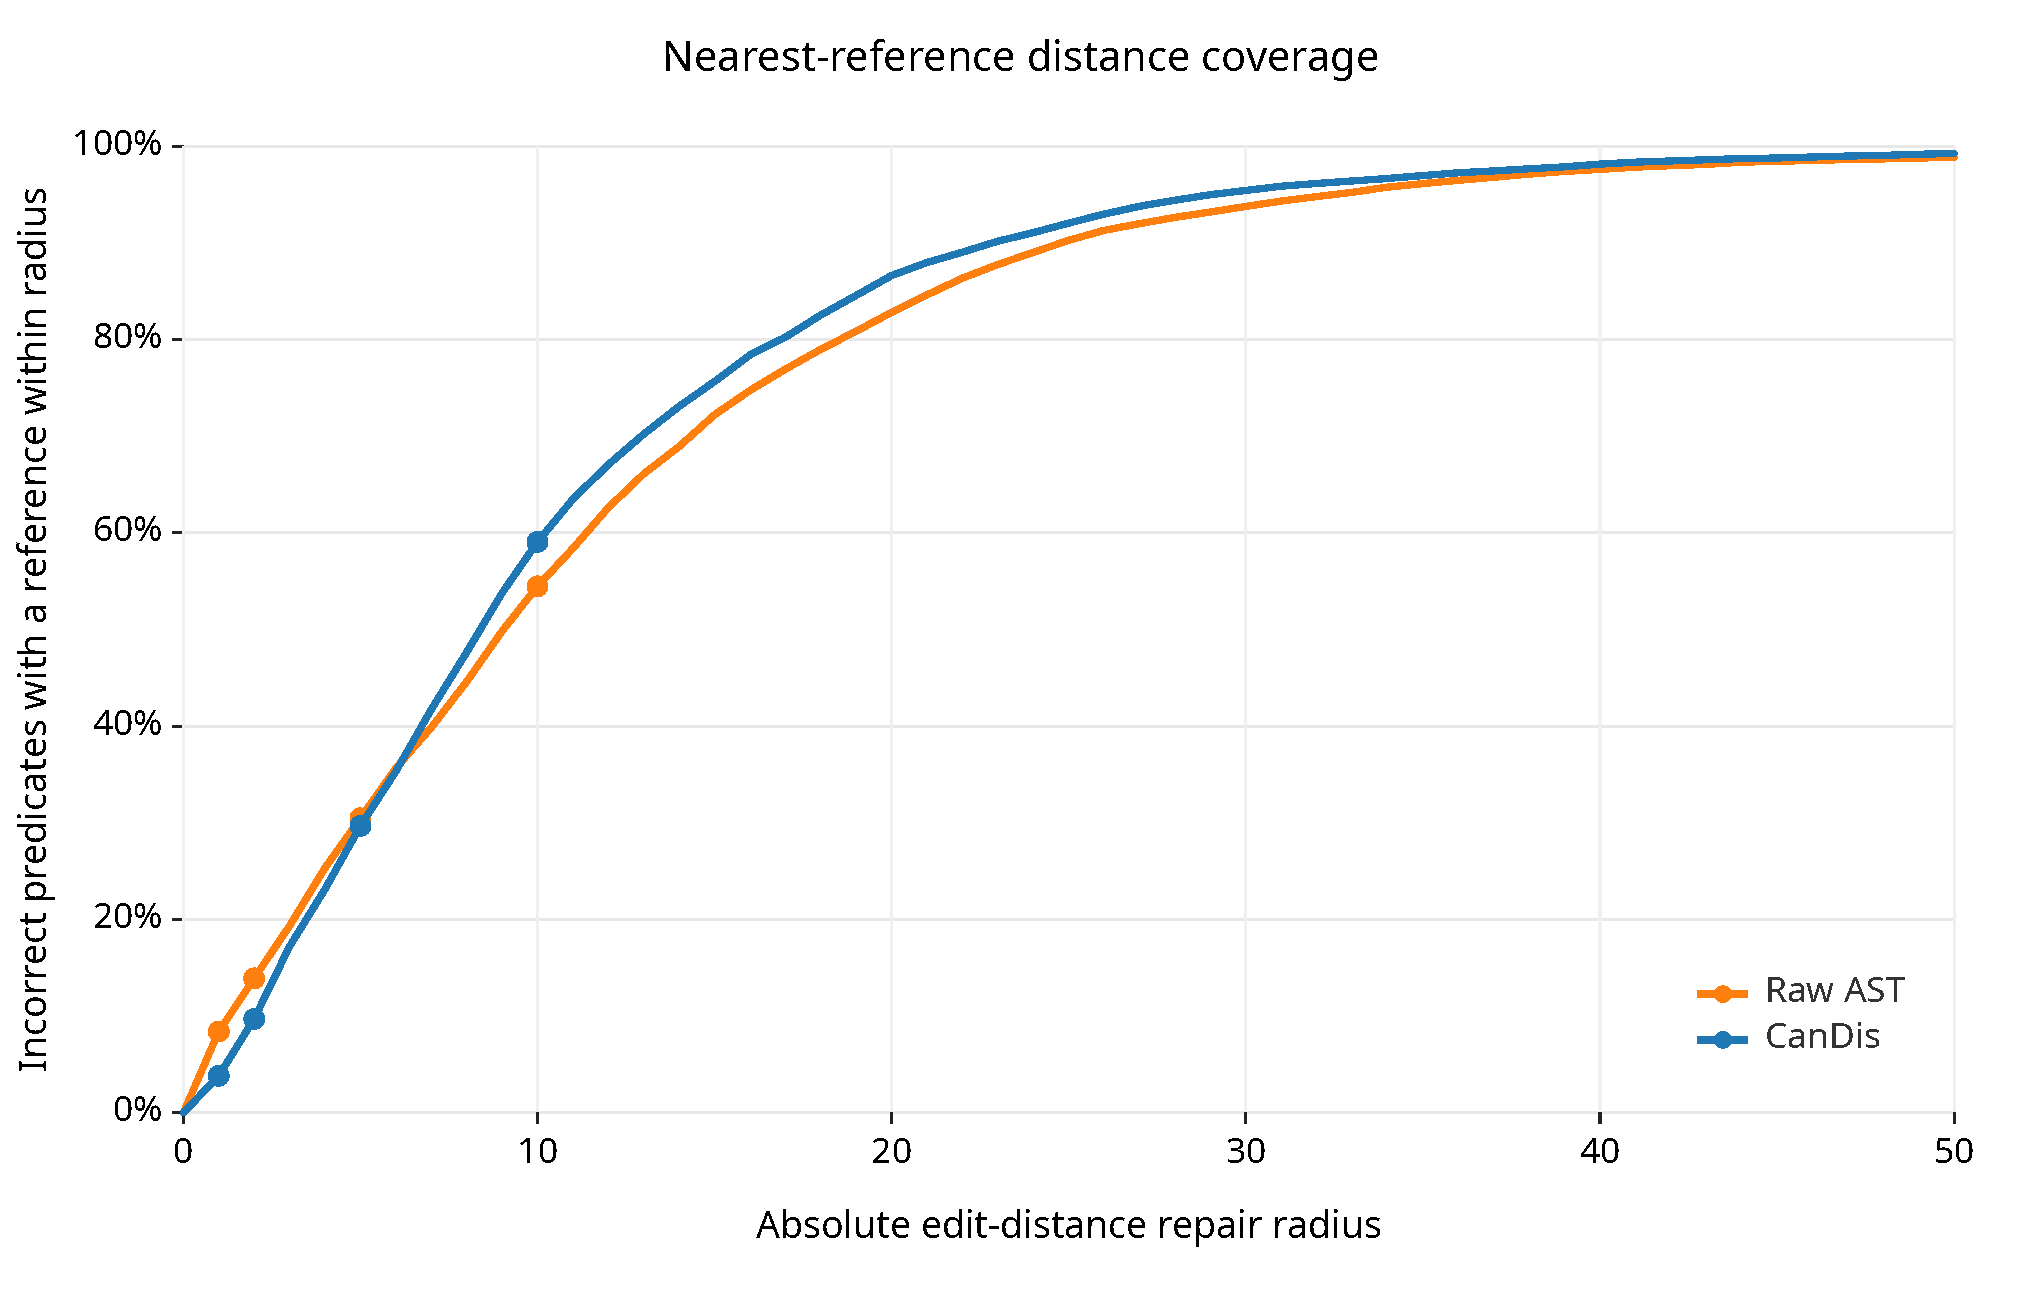
\includegraphics[width=0.82\linewidth]{figures/historical_repair_coverage.pdf}
\caption{Cumulative nearest-reference coverage for 42,386 incorrect
submissions. At an integer radius $r$, each curve counts submissions whose
nearest distinct-AST reference lies within $r$ edits under that metric.
All submissions remain in the denominator through the plotted limit of 50.}
\label{fig:distance-coverage}
\end{figure}


Figure~\ref{fig:distance-coverage} counts each submission once per metric
at each inclusive edit radius. At ten edits, 23,087 submissions had a raw-AST
reference within reach and 25,036 had a \CanDis{} reference within reach.
The two metrics can select different nearest references.

\subsection{What does checking a particular Alloy command add?}
\label{sec:scoped-pools}

A structural rewrite must hold wherever its key is reused. For instance, the
v3.1 rule moving a universal quantifier across \texttt{always} requires a
static domain: a later state must not introduce an atom that was absent at
the time of quantification. The five further rule families compare selected
relation rows or columns, bounded relation differences, ordinary and mixed
role selections, and threshold classifiers. Their conclusions need not survive
a change of command. With four-bit signed integers, for example, eight
predecessors are enough to make a count wrap negative. The test
\texttt{\#succs.t > 1} then fails although \texttt{not lone succs.t} holds.

The default comparison distinguishes structural equality from equality under
a fixed check of the two predicates. The latter test uses the resolved field,
binder and temporal frame, the effective carrier bounds and the actual integer
width. A match must produce the same witness in both orientations and the
native solver must find no counterexample. An \textsc{unsat} result without a
rule is not a new edge. For references from different files, the comparison
first checks that the relocated predicates retain their typed definitions,
imports, facts and compatible command bounds. It never substitutes a scoped
edge for an edit trace or writes that edge into the structural canonical key.

Every eligible student--oracle pair had a fixed command. A rule matched
347 pairs, recognizing 259 correct pairs beyond structural
equality. Across the 132,032 pairs of correct references every comparison
had a common command context and 1,234 pairs matched a rule.

To count \emph{structural forms}, we connect references in an invariant pool
when they have structural distance zero and count the connected components.
For \emph{fixed-command components}, we add the verified command-specific
edges and count again. A single new edge can join two entire components. The 4,496 references reduced to 1,816 structural forms
and then to 1,743 fixed-command components. Both paths recognized
all 8,952 original Slotted reference zeros and 10,319 more,
for 19,271 direct structural zeros.

\paragraph{Historical retention and native replay.}
The archives through v3.3 contain \histPublishedPaired{} distinct student--oracle
pairs and \histPublishedRefs{} direct reference pairs that reached zero in at
least one edition. Both paths retained every such pair. The regression test
checks each pair by its source and predicate identities in both engines. The 105 historical Alloy
counterexamples remained in separate fixed-command components. Seven CV
pairs had lost their shared structural form in v3.3. The repaired rules
cover these cases, including empty carriers, and each equivalence has a Lean proof.

The native checker replayed the edits selected by each engine from its
frozen normalized inputs. The ordered actions or temporal block effects
agreed on all 61,598 student--oracle comparisons, all 19,271
zero-distance reference pairs and 4,138 positive-distance ranking
comparisons selected for alternating quantifiers. Previously, completing a
partial binder map could displace an equally cheap ordinary alignment. Both
engines now break these ties by the surviving declaration positions. The
83 affected comparisons also agreed in reverse. A separate sample of one
paid comparison from each of the 181 pools agreed throughout.


\subsection{Which capabilities separate \CanDis{} from the baselines on controlled and natural predicates?}
\label{sec:eval-capability}

The seven-arm natural experiment found 5,137 correct zeros on each
\CanDis{} path, including all 2,228 Slotted zeros and 2,909
additional pairs. On the controlled suite, Slotted and both \CanDis{}
paths recognized all 5,500 transformations.

\begin{table}[t]
\centering
\caption{Natural-corpus effectiveness (19,212 correct and 42,386
incorrect distinct-AST pairs) and controlled capability coverage
(11 families of 500, including binder permutation).}

\label{tab:eval-effectiveness}
\scriptsize
\setlength{\tabcolsep}{2.7pt}
\begin{tabular}{@{}lrrrrr@{}}
\toprule
Arm & Correct $d=0$ & Incorrect $d=0$ & Mean dist. & Cap.\ All & Binder Perm.\\
\midrule
Raw & 820 (4.268\%) & 0 & 16.606 & 2,585/5,500 & 1/500\\
Raw + De Bruijn & 2,160 (11.243\%) & 0 & 16.145 & 3,628/5,500 & 22/500\\
Java egglog & 820 (4.268\%) & 0 & 16.477 & 2,585/5,500 & 1/500\\
Java egglog + De Bruijn & 2,160 (11.243\%) & 0 & 16.018 & 3,628/5,500 & 22/500\\
Slotted & 2,228 (11.597\%) & 0 & 16.324 & 5,500/5,500 & 500/500\\
\CanDis{} & 5,137 (26.738\%) & 0 & 13.471 & 5,500/5,500 & 500/500\\

\bottomrule
\end{tabular}
\end{table}

For the 5,137 distinct natural zero claims, bounded Alloy checks
found no counterexample under the recorded commands. All seven arms rejected
the 4 negative probes. The capability study checked 29 sampled
transformations against their source models.

\subsection{When do types reduce the cost of searching binder renamings?}
\label{sec:eval-synthetic}

\textbf{Answer:} Types reduce renaming search cost when they partition $N$
bindings across multiple types into smaller permutation groups
($\prod_{j=1}^M n_j!$ rather than $N!$); when all $N$ bindings share a single
type ($M=1$), typing yields no partition reduction. This synthetic benchmark is a
representation-construction runtime experiment comparing typed versus untyped
slots, not a comparison between the Fast Rewrite and Certificate-Integrated
implementations.

As explained in Section~\ref{sec:canonicalization-procedure}, exact
canonicalization enumerates $\prod_\tau |\Delta_{n,\tau}|!$ bijections across
typed slot fibres. For $N=10$ bindings, $M=1$ type leaves the full
$10!=3{,}628{,}800$ search space in both arms, whereas partitioning evenly across
$M=2$ types cuts the permutation count to $5!\,5!=14{,}400$ ($252\times$ fewer),
and $M=10$ distinct types reduces it to~$1$.

The historical v3 experiment evaluated this mechanism on a complete synthetic grid of \textbf{270} paired
predicates (\textbf{540} predicates, \textbf{1,080} trials) spanning
$N\in\{2,\dots,10\}$ outer bindings and $M\in\{1,\dots,N\}$ types (54 cells, 10
predicates per cell per arm; 8 isolated workers, 768\,MiB heap per JVM, and a
\textbf{300-second} deadline per predicate per arm; zero errors or unattempted
trials). Typed slots completed \textbf{530/540} trials (98.15\%, 10 timeouts),
versus \textbf{442/540} untyped (81.85\%, 98 timeouts). Every single timeout in
both arms occurred at $N=10$ bindings: all \textbf{10} typed timeouts occurred
at \textbf{10 bindings and one type}, while all \textbf{450/450} multi-type
typed trials completed, including \textbf{90/90} at 10 bindings ($M\ge 2$). In
the untyped arm, all 98 timeouts occurred at $N=10$ (2/10 succeeded at
$M=2$; 0/10 in the other nine $N=10$ cells). All timeouts are retained as
censored runtime observations rather than failures or omitted inputs.

\begin{figure}[tbp]
\centering
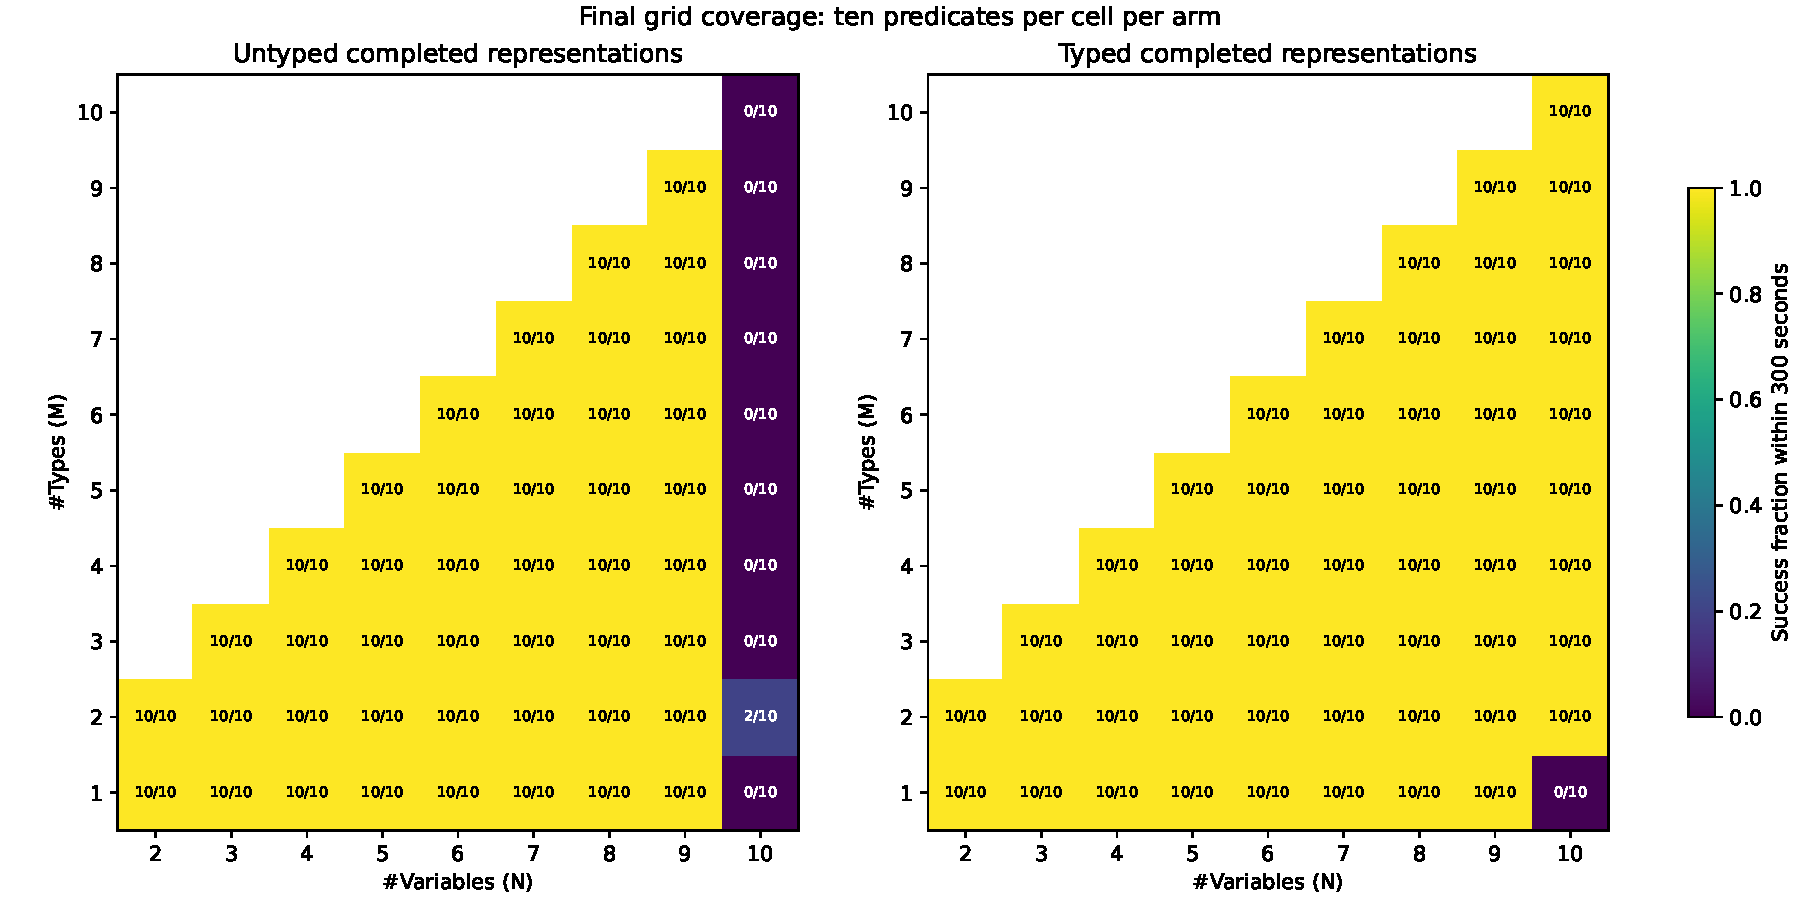
\includegraphics[width=0.94\linewidth]{figures/completion-grid.pdf}
\vspace{2pt}

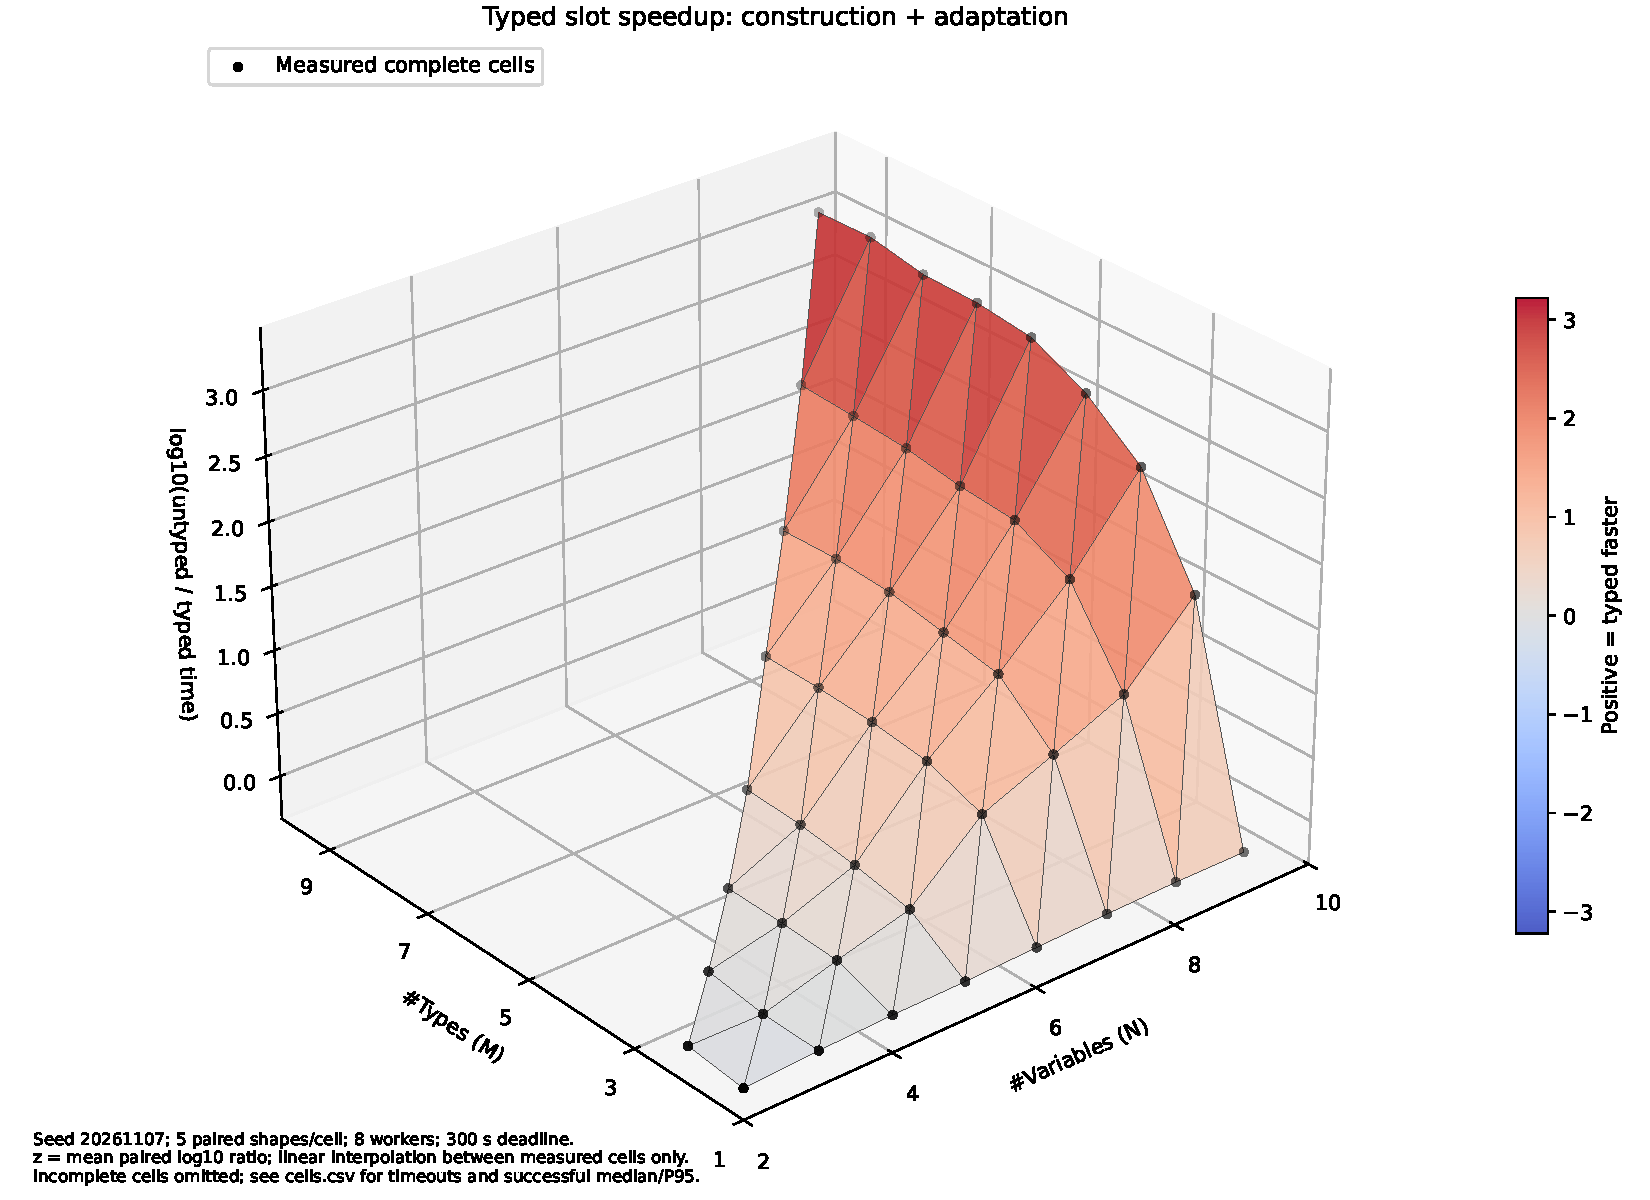
\includegraphics[width=0.72\linewidth]{figures/engine-speedup-surface.pdf}
\caption{Synthetic typed-versus-untyped scaling grid (540 predicates, 300\,s
deadline, 5 paired shapes per cell). \textbf{Top:} completion counts per
$(N,M)$ cell; all 10 typed timeouts are at $(10,1)$ and all 98 untyped timeouts
are at $N=10$. \textbf{Bottom:} mean $\log_{10}(\text{untyped}/\text{typed})$
engine elapsed time across the 44/54 complete matched cells without
interpolating across missing censored cells.}
\label{fig:synthetic-grid}
\end{figure}

On the same \textbf{442} jointly successful predicates, the ratio of untyped to
typed medians was \textbf{26.62$\times$} for engine elapsed time (0.670026\,s
vs.\ 0.025169\,s) and \textbf{5.12$\times$} for end-to-end elapsed time
(0.849457\,s vs.\ 0.166021\,s). These figures are ratios of medians over the
442 matched concurrent elapsed measurements, not medians of pairwise speedups,
CPU times, or timeout-inclusive estimates. Figure~\ref{fig:synthetic-grid}
displays the completion grid and the engine speedup surface across the 44/54
complete matched cells without interpolating missing cells (the end-to-end
surface and per-$N$ summary appear in Appendix~\ref{app:evaluation-detail}).

In the current natural slot-typing comparison, untyped and typed slots each recognized 2,228 pairs. Summed engine CPU time was 18.560\,s and 10.343\,s, respectively.

\subsection{What is the runtime and memory cost of certificate integration?}
\label{sec:eval-cost}

Fast Rewrite completed the natural arm in 27.910\,s with
2,059.3\,MiB maximum RSS. Certificate-Integrated took 386.579\,s
and 8,638.9\,MiB. These times cover each structural-ablation arm.
The paired and reference-pool runners also compare applicable Alloy commands.

\begin{table}[t]
\centering
\caption{Natural-ablation study runtime and memory across the five distinct
baselines and the two \CanDis{} implementations ($n=61{,}598$ eligible pairs).}
\label{tab:eval-runtime}
\scriptsize
\setlength{\tabcolsep}{2.1pt}
\begin{tabular}{@{}lrrrrr@{}}
\toprule
Arm & Arm Wall (s) & Eng.\ CPU (s) & Max File (s) & Peak Heap & Max RSS\\
& & & & (MiB) & (MiB)\\
\midrule
Raw & 17.531 & 3.842 & 0.158 & 696.1 & 1,347.6\\
Raw + De Bruijn & 17.788 & 4.862 & 0.139 & 728.8 & 1,381.8\\
Java egglog & 17.633 & 3.725 & 0.132 & 732.7 & 1,391.4\\
Java egglog + De Bruijn & 17.699 & 4.659 & 0.159 & 711.5 & 1,383.2\\
Slotted & 18.292 & 25.556 & 2.194 & 1,097.1 & 1,963.1\\
\CanDis{} (Fast Rewrite) & 27.910 & 151.309 & 0.384 & 1,027.1 & 2,059.3\\
\CanDis{} (Cert.-Integrated) & 386.579 & 5,512.368 & 3.962 & 6,303.3 & 8,638.9\\

\bottomrule
\end{tabular}
\end{table}

Table~\ref{tab:eval-runtime} reports one fresh process per arm.
The in-process checks and rebuilds give Certificate-Integrated a higher cost.
The study did not profile the share attributable to each operation.

\subsection{Scope and limitations}
\label{sec:eval-limits}

The Lean results address the abstract graph model. The Java results are
supported by in-process certificate checks, bounded native-operation
comparisons and the archived Alloy checks. Public operation witnesses and
end-to-end Java-to-Lean refinement remain open. The inherited labels and
recorded bounds limit the Alloy case study. The corpus contains 4,482
AST-identical paired rows and 21 cross-file raw-AST-identical reference
comparisons outside the distance measurements. Fresh-process timing
comes from a single run per ablation arm. The historical synthetic grid
preserves censored observations in cells where a trial reached its deadline.

\section{Conclusion}
\label{sec:conclusion}

Typed flexible-arity slotted e-graphs separate an expression's effective
support from its placement in the caller's context. In the abstract model,
complete finite quotient presentations yield exact canonical shapes.
Structural realization and compatible collisions preserve source equations,
and locally coherent updates give sound judgments between finite unfoldings.

Both Alloy rewrite paths retained every archived structural zero. They
recognized 2,909 correct student--oracle pairs beyond original Slotted and
assigned zero to no incorrect submission. Fixed-command rules recognized
259 further correct pairs. Repairing \replayOriginalFailures{} equal-cost
disagreements brought the ordered native replays into agreement on all
\replayPairs{} ranking pairs. The synthetic grid also shows how heterogeneous
slot types reduce the cost of searching binder renamings.

\label{end:main-text}

\clearpage
\label{start:references}
\bibliographystyle{splncs04}
\bibliography{ref}
\ifdefined\FullDraft
\appendix
\raggedbottom
\clearpage
\section{Supporting Calculations, Lean Correspondence, and Verification Scope}
\label{app:formal-details}

The main paper proves the four core theoretical results over the abstract
formal model. This appendix provides the two elementary calculations referenced
in Sections~\ref{sec:background} and~\ref{sec:formalism}, the exact
paper-to-theorem map and proof dependency structure against the Lean~4.33.0
development at tag \texttt{v3}, the remaining formalized lemmas, and the exact
boundary between formal proofs and Java implementation checks.

\subsection{Supporting Calculations}

\paragraph{Size of binary AC closure.}
Take $n$ distinct generators with no unit or additional equations. Square-free
subproducts correspond to nonempty subsets of generators, yielding $2^n-1$
classes. An ordered binary node corresponds to a pair of nonempty disjoint
subsets: each generator is placed on the left, on the right, or in neither.
Of the $3^n$ ternary assignments, $2^n$ leave the left side empty and $2^n$
leave the right side empty, overlapping on the single all-absent assignment.
Adding that overlap back yields $3^n+1-2^{n+1}$ ordered binary nodes.

\paragraph{Changing caller names.}
Suppose two leader invocations align via
$\rho\circ\widehat m=\widehat m'\circ\pi$. After caller renamings $\eta$ and
$\eta'$, the alignment transports via conjugation
$\bar\rho=\eta'\circ\rho\circ\eta^{-1}$ because
\[
 \bar\rho\circ\eta\circ\widehat m
 =\eta'\circ\rho\circ\widehat m
 =\eta'\circ\widehat m'\circ\pi.
\]
When $\rho$ is the identity, $\widehat m=\widehat m'\circ\pi$. Because $\pi$ is
a bijection, $\operatorname{im}(\widehat m)=\operatorname{im}(\widehat m')$, so
any justified leader symmetry preserves the set of caller slots used.

\subsection{Paper-to-Theorem Map and Proof Dependencies}

Table~\ref{tab:lean-correspondence} maps each main-text result (plus the
typed-slot partitioning property underlying Section~\ref{sec:eval-synthetic})
to its exact file path and Lean declaration name(s) in the \texttt{v3}
repository. Table~\ref{tab:lean-remaining} records the remaining supporting
formal results.

\begin{table}[ht]
\centering
\caption{Paper-to-theorem map against the Lean development at tag
\texttt{v3}. Module paths under \texttt{TypedSlottedEGraphsPaper/} live in
\texttt{paper-claims/formal/TypedSlottedEGraphsPaper/}.}
\label{tab:lean-correspondence}
\scriptsize
\setlength{\tabcolsep}{2.2pt}
\begin{tabular}{@{}%
>{\raggedright\arraybackslash}p{3.0cm}%
>{\raggedright\arraybackslash}p{3.0cm}%
>{\raggedright\arraybackslash}p{5.75cm}@{}}
\toprule
Paper result & Repository file (\texttt{v3}) & Exact Lean declaration(s)\\
\midrule
Theorem~\ref{thm:shape-exactness}: Effective-support canonical-shape exactness &
\texttt{TypedSlottedEGraphs\allowbreak Paper/\allowbreak Normalization\allowbreak Bridge.lean} &
\texttt{AmbientQuotient\allowbreak Presentation.\allowbreak ambientQuotientNormal\allowbreak FormExactness},
\texttt{EffectiveSupport\allowbreak Canonicalizer.\allowbreak effectiveSupportCanonical\allowbreak ShapeExactness},
\texttt{EffectiveSupport\allowbreak Canonicalizer.\allowbreak canonicalRecord\allowbreak Postconditions}\\[4pt]
Proposition~\ref{thm:structural-soundness}: Structural realization and congruence soundness &
\texttt{TypedSlottedEGraphs\allowbreak Paper/\allowbreak StructuralContainer\allowbreak Adapter.lean};
\texttt{Structural\allowbreak Semantics.lean} &
\texttt{concreteTypedAlpha\allowbreak SemanticSoundness},
\texttt{concretePortAndNode\allowbreak CongruenceCertificate},
\texttt{concretePortAndNode\allowbreak CongruenceSemanticSoundness},
\texttt{StructuralRealizer.\allowbreak structuralRealizationNaturality},
\texttt{structuralAlphaBinderBlock\allowbreak SemanticSoundness},
\texttt{structuralPortAndNode\allowbreak CongruenceSoundness}\\[4pt]
Proposition~\ref{thm:collision-soundness}: Compatible effective-shape collisions &
\texttt{TypedSlottedEGraphs\allowbreak Paper/\allowbreak TheoremBridge.lean} &
\texttt{paperF25CertifiedLeader\allowbreak KernelExtraction},
\texttt{canonicalEqualityYields\allowbreak KernelCollision},
\texttt{paperF26CertifiedEffective\allowbreak ShapeCollision},
\texttt{paperAtom038Ambient\allowbreak CollisionCertificate}\\[4pt]
Theorem~\ref{thm:semantic-sound}: Certificate-preserving reachability and finite-unfolding soundness &
\texttt{TypedSlottedEGraphs\allowbreak Paper/\allowbreak TheoremBridge.lean};
\texttt{Reachability.lean}; \texttt{TraceSemantics.lean} &
\texttt{paperF24FindAndFinite\allowbreak UnfoldingPreserve\allowbreak EquationalCertificates},
\texttt{paperF27CertificatePreserving\allowbreak ReachabilityAndFinite\allowbreak UnfoldingSoundness},
\texttt{certificatePreserving\allowbreak ReachabilityAndFinite\allowbreak UnfoldingSoundness},
\texttt{obligationAddition\allowbreak PreservesCoherence},
\texttt{obligationRekey\allowbreak PreservesCoherence},
\texttt{obligationRemoval\allowbreak PreservesCoherence},
\texttt{obligationComposition\allowbreak PreservesCoherence}\\[4pt]
Section~\ref{sec:eval-synthetic}: Typed-slot partition search &
\texttt{docs/slot-typing-\allowbreak ablation/\allowbreak Partitioned\allowbreak Permutation.lean} &
\texttt{PartitionedPermutation.\allowbreak generated\_\allowbreak preserves\_\allowbreak key},
\texttt{PartitionedPermutation.\allowbreak generated\_\allowbreak rejects\_\allowbreak cross\_\allowbreak partition},
\texttt{PartitionedPermutation.\allowbreak every\_\allowbreak preserving\_\allowbreak mapping\_\allowbreak is\_\allowbreak represented}\\
\bottomrule
\end{tabular}
\end{table}

\begin{table}[ht]
\centering
\caption{Remaining formalized Lean results at tag \texttt{v3}.}
\label{tab:lean-remaining}
\scriptsize
\setlength{\tabcolsep}{2.2pt}
\begin{tabular}{@{}%
>{\raggedright\arraybackslash}p{2.95cm}%
>{\raggedright\arraybackslash}p{3.05cm}%
>{\raggedright\arraybackslash}p{5.75cm}@{}}
\toprule
Topic & Repository file (\texttt{v3}) & Exact Lean declaration(s)\\
\midrule
Binary AC closure counts &
\texttt{TypedSlottedEGraphs\allowbreak Paper/\allowbreak ACClosureCounts.lean} &
\texttt{ACClosureCounts.\allowbreak completeBinary\allowbreak ACClosureCounts},
\texttt{ACClosureCounts.\allowbreak sizeOfComplete\allowbreak BinaryACClosure}\\[3pt]
Category, support, rebuild quiescence &
\texttt{TypedSlottedEGraphs\allowbreak Paper/\allowbreak StructuralClaims.lean} &
\texttt{typedEmbedding\allowbreak CategoryLaws},
\texttt{leaderization\allowbreak ContractsSupport},
\texttt{finiteRebuildQuiescence}\\[3pt]
Concrete support and invocation safety &
\texttt{TypedSlottedEGraphs\allowbreak Paper/\allowbreak SyntaxSupport.lean} &
\texttt{concreteTypedEmbeddings\allowbreak PreserveTypes},
\texttt{concreteSlotSupportInvariance},
\texttt{concreteTypeSafety\allowbreak OfInvocation}\\[3pt]
Parent forest and collision index &
\texttt{TypedSlottedEGraphs\allowbreak Paper/\allowbreak ContextGraph.lean} &
\texttt{FiniteTypedParentForest.\allowbreak find\_\allowbreak support\_\allowbreak contracts},
\texttt{QuiescentFiniteTypedEGraph.\allowbreak graphInvocation\allowbreak Alignment\_\allowbreak transport},
\texttt{QuiescentFiniteTypedEGraph.\allowbreak identityAligned\allowbreak LeaderSupport},
\texttt{F10FiniteQuiescentGraph\allowbreak Environment.\allowbreak collisionIndexExact}\\[3pt]
Source rule laws and arithmetic profile &
\texttt{TypedSlottedEGraphs\allowbreak Paper/\allowbreak ProfileRules.lean} &
\texttt{tsgRule012\_\allowbreak phaseLocalPrenex\allowbreak AndDomainGuarding}--\texttt{tsgRule019\_\allowbreak implicationLocalSaturation},
\texttt{tsgCe003\_\allowbreak overflowReassociation\allowbreak Counterexample},
\texttt{tsgScope001\_\allowbreak zeroCanonical\allowbreak DistanceBoundary}\\[3pt]
Worked abstract trace witness &
\texttt{TypedSlottedEGraphs\allowbreak Paper/\allowbreak TraceEnvelope\allowbreak Witness.lean} &
\texttt{TraceEnvelopeWitness.\allowbreak d1\_\allowbreak trace\_\allowbreak obligation},
\texttt{TraceEnvelopeWitness.\allowbreak d2\_\allowbreak trace\_\allowbreak obligation},
\texttt{TraceEnvelopeWitness.\allowbreak machineChecked\allowbreak EndToEndWitness}\\[3pt]
Slot-typing grid \& negative controls &
\texttt{docs/slot-typing-\allowbreak ablation/\allowbreak Model.lean}, \texttt{BalancedGrid.lean}, \texttt{Independent\allowbreak BindingBlocks.lean} &
\texttt{different\_\allowbreak sorts\_\allowbreak distinct}, \texttt{erasure\_\allowbreak can\_\allowbreak collide},
\texttt{typed\_\allowbreak mappings\_\allowbreak subset}, \texttt{allocation\_\allowbreak total}, \texttt{balanced},
\texttt{mixed\_\allowbreak quantifier\_\allowbreak exchange\_\allowbreak is\_\allowbreak invalid},
\texttt{dropping\_\allowbreak disjointness\_\allowbreak is\_\allowbreak invalid},
\texttt{moving\_\allowbreak all\_\allowbreak across\_\allowbreak eventually\_\allowbreak is\_\allowbreak invalid}\\[3pt]
Source normalization scheduling &
\texttt{docs/distance-parity-\allowbreak 20261107/\allowbreak CapabilitySource\allowbreak Scheduling.lean} &
\texttt{membership\_\allowbreak before\_\allowbreak distribution},
\texttt{subcarrier\_\allowbreak membership\_\allowbreak elimination},
\texttt{restriction\_\allowbreak universal\_\allowbreak neutral},
\texttt{empty\_\allowbreak domain\_\allowbreak guard\_\allowbreak retained},
\texttt{disjoint\_\allowbreak declarations\_\allowbreak retained}\\
\bottomrule
\end{tabular}
\end{table}

\paragraph{Module dependency structure and trusted computing base.}
The main formal development under \texttt{paper-claims/formal/} has an acyclic
module graph:
\begin{quote}\small
\texttt{Core} $\to$ \{\texttt{SyntaxSupport}, \texttt{ContextGraph},
\texttt{Certificates}\}\\
$\to$ \{\texttt{FiniteNormalization} $\to$ \texttt{NormalizationBridge},\\
\hspace*{1.2em}\texttt{StructuralSemantics} $\to$ \texttt{StructuralContainerAdapter},\\
\hspace*{1.2em}\texttt{TraceSemantics} $\to$ \texttt{Reachability}\}\\
$\to$ \texttt{TheoremBridge} $\to$ \texttt{ClaimLedger} / \texttt{PaperIndex}.
\end{quote}
Across the audited Lean~4.33.0 development (\texttt{tcb-manifest.json}
under \texttt{paper-claims/formal/}),
the 146 active mapped units depend solely on Lean's standard foundational
axioms (\texttt{propext}, \texttt{Quot.sound}, \texttt{Classical.choice}),
with zero project-defined axioms, zero \texttt{sorry} placeholders, and zero
\texttt{native\_decide} or unsafe dependencies.

\subsection{Formal Proofs vs.\ Implementation Checks and Empirical Evidence}

To keep formal and empirical claims distinct:
\begin{itemize}
\item \textbf{Formal-model theorems} (Table~\ref{tab:lean-correspondence})
  establish exactness, realization soundness, collision soundness, and
  coherence-preserving finite-unfolding soundness over the Lean abstract
  model, plus one concrete machine-checked abstract trace in
  \texttt{TraceEnvelopeWitness}.
\item \textbf{Java implementation checks} consist of (i)~in-process
  strict-every-transition invariant and certificate checks in
  Certificate-Integrated IR, (ii)~an independent Java certificate verifier and
  adversarial suite covering support contraction, collision, union, symmetry,
  rebuilding, path compression, container laws, binder orbits, and incomplete
  evidence, (iii)~the native-operation comparison across all 61,598 eligible
  paired comparisons (0 mismatches, 0 unchecked, 0 invalid replays, 0 errors),
  and (iv)~bounded Alloy checks on the union of 4,499 natural zero claims and
  29 capability subtype checks.
\item \textbf{Open verification boundary:} The native-operation comparator
  authenticates its \texttt{FROZEN\_NORMALIZED\_IR} boundary, while general
  Java-to-Lean correspondence (\texttt{javaLeanCorrespondence\allowbreak Checked}),
  source-to-certificate wire replay (\texttt{sourceCertificateWire\allowbreak ReplayChecked}),
  and public repair-sequence linkage (\texttt{publicSequenceLinked}) remain
  open. Likewise, observed zero-discrepancy agreement between Fast Rewrite and
  Certificate-Integrated IR is an empirical check on the evaluated workloads,
  not a universal equivalence theorem.
\end{itemize}

\paragraph{Source rewrites added in v3.1.}
In \path{docs/section3-repair-audit/formal/Phase5SourceRules.lean},
\path{unary_restrictions_are_intersection} treats unary restrictions, and
\path{unary_image_of_domain_restriction} handles the typed join boundary.
\path{static_all_commutes_with_always} fixes the domain across time;
\path{changing_domain_blocks_all_always} refutes the unrestricted law.
\path{next_fixed_binding_observation} keeps the bound value fixed and primes
the observed carrier. The subdomain and difference lemmas restrict the
binding at its original instant. These are results about the formal source
semantics, not a proof of the whole Java frontend.

\clearpage
\section{Experimental Detail}
\label{app:evaluation-detail}

The following appendix preserves the v3.3 natural-corpus, reference-pool,
runtime and capability tables and by-invariant plots from 26 November 2026.
The current measurements are in Section~\ref{sec:evaluation}. The synthetic
scaling study comes from v3 and retains its 300-second deadline.

\subsection{Pipeline Variants}

\begin{table}[H]
\caption{Representation and equality discovery across the five distinct
baselines and the two \CanDis{} implementations.}
\label{tab:engine-boundary}
\centering
\scriptsize
\setlength{\tabcolsep}{3pt}
\begin{tabular}{@{}%
>{\raggedright\arraybackslash}p{2.45cm}%
>{\raggedright\arraybackslash}p{2.7cm}%
>{\raggedright\arraybackslash}p{3.05cm}%
>{\raggedright\arraybackslash}p{3.25cm}@{}}
\toprule
Arm & Stored form & Equality discovery & Role\\
\midrule
Raw & ordered fixed-arity keys & bounded concrete rewrite frontier & fixed-arity baseline\\
Raw + De Bruijn & fixed keys with DB leaves & same frontier & binding encoding added\\
Java egglog & flattened concrete keys & same frontier & variadic internal baseline\\
Java egglog + De Bruijn & flattened keys with DB leaves & same frontier & combined internal baseline\\
Slotted & ordered invocations and integer slots & frontier plus bounded slot canonicalizer & untyped slot-aware baseline\\
\CanDis{} (Fast Rewrite) & flexible Alloy repair view & staged normalization and reference metric & high-throughput canonical path\\
\CanDis{} (Cert.-Integrated) & typed $\Seq/\Bag/\Set/\texttt{One}$ ports & certified graph, orbit, rebuild, finite unfolding & in-process certificate and invariant checks\\
\bottomrule
\end{tabular}
\end{table}

\newcommand{\invariantpanel}[3]{%
\begin{figure}[H]\centering
\includegraphics[page=#1,width=\linewidth]{figures/forms-by-invariant.pdf}
\caption{#2. Each row reports raw unique ASTs, v3.3 structural forms and v3.3 fixed-command components for that invariant, in that order. Bar lengths share a scale
within each problem; the numbers give the exact counts.}\label{#3}
\end{figure}}
\invariantpanel{1}{Unique forms by invariant: classroom, courses, and CV}{fig:scoped-by-invariant}
\invariantpanel{2}{Unique forms by invariant: graphs, LTS, production lines, and social media}{fig:scoped-by-invariant-middle}
\invariantpanel{3}{Unique forms by invariant: train stations and trash}{fig:scoped-by-invariant-last}


\subsection{Representation Sizes, Truth Pools, and Distance Distributions}

\begin{table}[H]
\centering
\caption{Mean of the larger endpoint size in each representation on the paired natural corpus
($n=61{,}598$ eligible distinct-AST pairs). Each view uses its own structural
units.}
\label{tab:compact}
\small
\begin{tabular}{@{}p{4.3cm}p{5.5cm}r@{}}
\toprule
View & Experimental role & Mean units\\
\midrule
Raw Alloy AST & source-level structural baseline & 19.669\\
\CanDis{} repair observation & editable view used by the repair metric & 17.893\\
\CanDis{} representative tree & deterministic finite tree for diagnostic TED & 33.187\\
\bottomrule
\end{tabular}
\end{table}

\begin{table}[H]\centering
\caption{Reference counts by problem. Each count sums forms within its invariant pools. A dash marks a problem with a missing command context.}
\label{tab:truth_metrics}\small\begin{tabular}{@{}lrrr@{}}\toprule
Problem & Raw ASTs & v3.3 structural & v3.3 fixed command\\\midrule
\texttt{classroom\_fol} & 279 & 88 & 84\\
\texttt{classroom\_rl} & 266 & 140 & 132\\
\texttt{coursesNew} & 408 & 192 & 181\\
\texttt{coursesOld} & 527 & 267 & 261\\
\texttt{cv\_v1} & 42 & 23 & 23\\
\texttt{cv\_v2} & 32 & 25 & 25\\
\texttt{graphs} & 224 & 112 & 111\\
\texttt{lts} & 105 & 56 & 56\\
\texttt{productionLineNew} & 249 & 116 & 115\\
\texttt{productionLine\_v1} & 58 & 44 & 43\\
\texttt{productionLine\_v2} & 354 & 194 & 194\\
\texttt{socialMedia} & 919 & 293 & 286\\
\texttt{trainStationNew} & 360 & 159 & 128\\
\texttt{trainStationOld} & 62 & 46 & 46\\
\texttt{trash\_fol} & 253 & 86 & 83\\
\texttt{trash\_ltl} & 157 & 74 & 74\\
\texttt{trash\_rl} & 201 & 101 & 100\\
\midrule
Total & 4,496 & 2,016 & 1,942\\
\bottomrule\end{tabular}\end{table}

\begin{table}[H]
\centering
\caption{Mean paired distance ($n=61{,}598$), nearest-reference distance
($n=42{,}386$, across 1,894,168 recorded comparisons), and inclusive
nearest-reference radius coverage. Coordinates use metric-specific edit units;
a dash indicates a diagnostic not computed on the Augmenter pool.}
\label{tab:distance-summary}
\scriptsize
\setlength{\tabcolsep}{3.5pt}
\begin{tabular}{@{}llcc@{}}
\toprule
Coordinate & Unit & Paired mean & Nearest-truth mean\\
& & ($n=61{,}598$) & ($n=42{,}386$)\\
\midrule
Levenshtein & characters & 39.261 & 28.055\\
Raw Alloy AST & AST nodes & 17.087 & 12.267\\
\CanDis{} & repair projection edits & 13.910 & 11.477\\
Representative TED & finite-tree edits & 32.137 & ---\\
\bottomrule
\end{tabular}

\medskip
\begin{tabular}{@{}lrrrr|lrrrr@{}}
\toprule
Abs.\ radius & \multicolumn{2}{c}{Raw AST} & \multicolumn{2}{c|}{\CanDis{}} &
Rel.\ radius & \multicolumn{2}{c}{Raw AST} & \multicolumn{2}{c}{\CanDis{}}\\
\midrule
$\le 1$ & 3,565 & (8.4\%) & 1,677 & (4.0\%) & $\le 5\%$ & 906 & (2.1\%) & 231 & (0.5\%)\\
$\le 2$ & 5,895 & (13.9\%) & 4,336 & (10.2\%) & $\le 10\%$ & 3,305 & (7.8\%) & 1,163 & (2.7\%)\\
$\le 5$ & 12,915 & (30.5\%) & 13,168 & (31.1\%) & $\le 20\%$ & 6,620 & (15.6\%) & 4,938 & (11.7\%)\\
$\le 10$ & 23,087 & (54.5\%) & 25,298 & (59.7\%) & $\le 50\%$ & 17,088 & (40.3\%) & 16,046 & (37.9\%)\\
\bottomrule
\end{tabular}
\end{table}


\subsection{Complete Natural Ablation and Controlled Capability Tables}

\begin{table}[H]
\centering
\caption{Complete natural-corpus ablation ($n=61{,}598$ eligible pairs out of
66,080 files; 4,482 AST-identical rows accounted separately; zero failures).
Effectiveness (top) reports one \CanDis{} row; runtime and memory (bottom)
distinguish Fast Rewrite from Certificate-Integrated IR in the natural ablation
study arm.}
\label{tab:ablation-natural}
\scriptsize
\setlength{\tabcolsep}{2.8pt}
\begin{tabular}{@{}lrrrrrr@{}}
\toprule
Arm & Correct $d=0$ & Incorr.\ $d=0$ & All avg & Corr.\ avg & Inc.\ avg & P50 / P95\\
\midrule
Raw & 820 (4.268\%) & 0 & 16.606 & 12.906 & 18.283 & 14 / 37\\
Raw + De Bruijn & 2,160 (11.243\%) & 0 & 16.145 & 12.508 & 17.794 & 14 / 36\\
Java egglog & 820 (4.268\%) & 0 & 16.477 & 12.811 & 18.139 & 14 / 36\\
Java egglog + De Bruijn & 2,160 (11.243\%) & 0 & 16.018 & 12.422 & 17.648 & 14 / 36\\
Slotted & 2,228 (11.597\%) & 0 & 16.324 & 12.638 & 17.995 & 14 / 37\\
\CanDis{} & 4,499 (23.418\%) & 0 & 13.910 & 9.078 & 16.100 & 11 / 34\\
\bottomrule
\end{tabular}

\medskip
\setlength{\tabcolsep}{1.3pt}
\begin{tabular}{@{}lrrrrrrr@{}}
\toprule
Arm & Arm Wall & Proc.\ Wall & Eng.\ CPU & Max File & Peak Heap & Max RSS & Mean\\
& (s) & (s) & (s) & (s) & (MiB) & (MiB) & units\\
\midrule
Raw & 18.233 & 18.700 & 3.284 & 0.113 & 802.4 & 1,532.9 & 39.154\\
Raw + De Bruijn & 18.765 & 19.230 & 4.121 & 0.132 & 727.9 & 1,418.7 & 39.142\\
Java egglog & 18.602 & 19.040 & 3.175 & 0.118 & 672.8 & 1,478.9 & 38.265\\
Java egglog + De Bruijn & 18.715 & 19.180 & 3.939 & 0.137 & 787.5 & 1,508.5 & 38.250\\
Slotted & 18.802 & 19.400 & 18.409 & 1.455 & 1,034.9 & 1,901.8 & 34.311\\
\CanDis{} (Fast Rewrite) & 26.683 & 27.130 & 141.496 & 0.362 & 1,067.9 & 2,115.7 & 29.339\\
\CanDis{} (Cert.-Integrated) & 398.186 & 398.760 & 5,676.430 & 3.697 & 6,483.8 & 8,595.6 & 29.339\\
\bottomrule
\end{tabular}

\parbox{0.97\linewidth}{\footnotesize\emph{Notes.} Peak Heap and Max RSS are in
MiB. Zero-set transitions: Raw$\to$Raw+DB $+1{,}340/-0$;
Java egglog$\to$Java egglog+DB $+1{,}340/-0$;
Java egglog+DB$\to$Slotted $+71/-3$; Slotted$\to$\CanDis{} $+2{,}271/-0$.}
\end{table}

\begin{table}[H]
\centering
\caption{Controlled capability benchmark across 11 transformation families of
500 pairs each (5,500 total pairs). Var.\ denotes the variadic Java egglog
core, DB denotes De Bruijn indexing, and \CanDis{} reports the shared recovery
across both canonical implementations.}
\label{tab:capability-benchmark}
\scriptsize
\setlength{\tabcolsep}{2.4pt}
\begin{tabular}{@{}lrrrrrr@{}}
\toprule
Transformation family (500 pairs) & Raw & Raw+DB & Var. & Var.+DB & Slotted & \CanDis{}\\
\midrule
Alpha-equivalence & 0 & 500 & 0 & 500 & 500 & 500\\
Associativity / commutativity / idempotence & 500 & 500 & 500 & 500 & 500 & 500\\
Binder-block permutations & 1 & 22 & 1 & 22 & 500 & 500\\
Safe prenex transformations & 500 & 500 & 500 & 500 & 500 & 500\\
Negation / logical normalization & 500 & 500 & 500 & 500 & 500 & 500\\
Temporal normalization & 500 & 500 & 500 & 500 & 500 & 500\\
Composed: $\alpha$ + AC & 0 & 500 & 0 & 500 & 500 & 500\\
Composed: $\alpha$ + binder permutation & 0 & 22 & 0 & 22 & 500 & 500\\
Composed: binder permutation + prenex & 22 & 22 & 22 & 22 & 500 & 500\\
Composed: AC + logical normalization & 500 & 500 & 500 & 500 & 500 & 500\\
Composed: mixed 2--4 transformations & 62 & 62 & 62 & 62 & 500 & 500\\
\midrule
All composed (5 families / 2,500 pairs) & 584 & 1,106 & 584 & 1,106 & 2,500 & 2,500\\
\textbf{All families (11 families / 5,500 pairs)} & 2,585 & 3,628 & 2,585 & 3,628 & 5,500 & 5,500\\
\bottomrule
\end{tabular}
\end{table}


\subsection{Natural Slot Typing and Synthetic Scaling Summary}

\begin{table}[H]
\centering
\caption{Typed versus untyped slots on the natural corpus (top, $n=61{,}598$)
and the synthetic scaling grid (bottom, 540 predicates, 300\,s deadline).
Synthetic medians use completed trials only; matched statistics use the 442
jointly successful predicates (matched P95 engine: 43.590\,s untyped vs.\
1.071\,s typed; end-to-end: 43.729\,s vs.\ 1.966\,s).}
\label{tab:typing-ablation}
\scriptsize
\setlength{\tabcolsep}{2.5pt}
\begin{tabular}{@{}lrrrrrrr@{}}
\toprule
Natural slot arm & Zeroes & Mean & Proc.\ Wall & Eng.\ CPU & Peak Heap & Max RSS & Source\\
& & dist. & (s) & (s) & (MiB) & (MiB) & slots\\
\midrule
\texttt{slotted-egraph} & 2,228 & 16.324 & 19.990 & 19.758 & 1,071.2 & 1,972.6 & 170,112\\
\texttt{slotted-egraph-typed} & 2,228 & 16.421 & 19.340 & 10.294 & 919.7 & 1,697.9 & 170,112\\
\bottomrule
\end{tabular}

\medskip
\setlength{\tabcolsep}{2.7pt}
\begin{tabular}{@{}lrrrrrrrr@{}}
\toprule
Bindings $N$ & Preds & \multicolumn{2}{c}{Completed} & \multicolumn{2}{c}{Med.\ engine (s)} & \multicolumn{2}{c}{Med.\ end-to-end (s)}\\
\cmidrule(lr){3-4}\cmidrule(lr){5-6}\cmidrule(lr){7-8}
& & Untyped & Typed & Untyped & Typed & Untyped & Typed\\
\midrule
2 & 20 & 20 (100\%) & 20 (100\%) & 0.013 & 0.016 & 0.166 & 0.166\\
3 & 30 & 30 (100\%) & 30 (100\%) & 0.015 & 0.017 & 0.166 & 0.166\\
4 & 40 & 40 (100\%) & 40 (100\%) & 0.023 & 0.018 & 0.166 & 0.166\\
5 & 50 & 50 (100\%) & 50 (100\%) & 0.044 & 0.021 & 0.201 & 0.166\\
6 & 60 & 60 (100\%) & 60 (100\%) & 0.199 & 0.024 & 0.366 & 0.166\\
7 & 70 & 70 (100\%) & 70 (100\%) & 0.720 & 0.027 & 0.866 & 0.166\\
8 & 80 & 80 (100\%) & 80 (100\%) & 3.688 & 0.031 & 3.985 & 0.166\\
9 & 90 & 90 (100\%) & 90 (100\%) & 36.353 & 0.033 & 36.505 & 0.167\\
10 & 100 & 2 (2\%) & 90 (90\%) & 265.145 & 0.034 & 265.282 & 0.166\\
\midrule
All & 540 & 442 (81.85\%) & 530 (98.15\%) & 0.670 & 0.026 & 0.849 & 0.166\\
Matched & 442 & 442 (100\%) & 442 (100\%) & 0.670 & 0.025 & 0.849 & 0.166\\
\bottomrule
\end{tabular}
\end{table}


\begin{figure}[H]
\centering
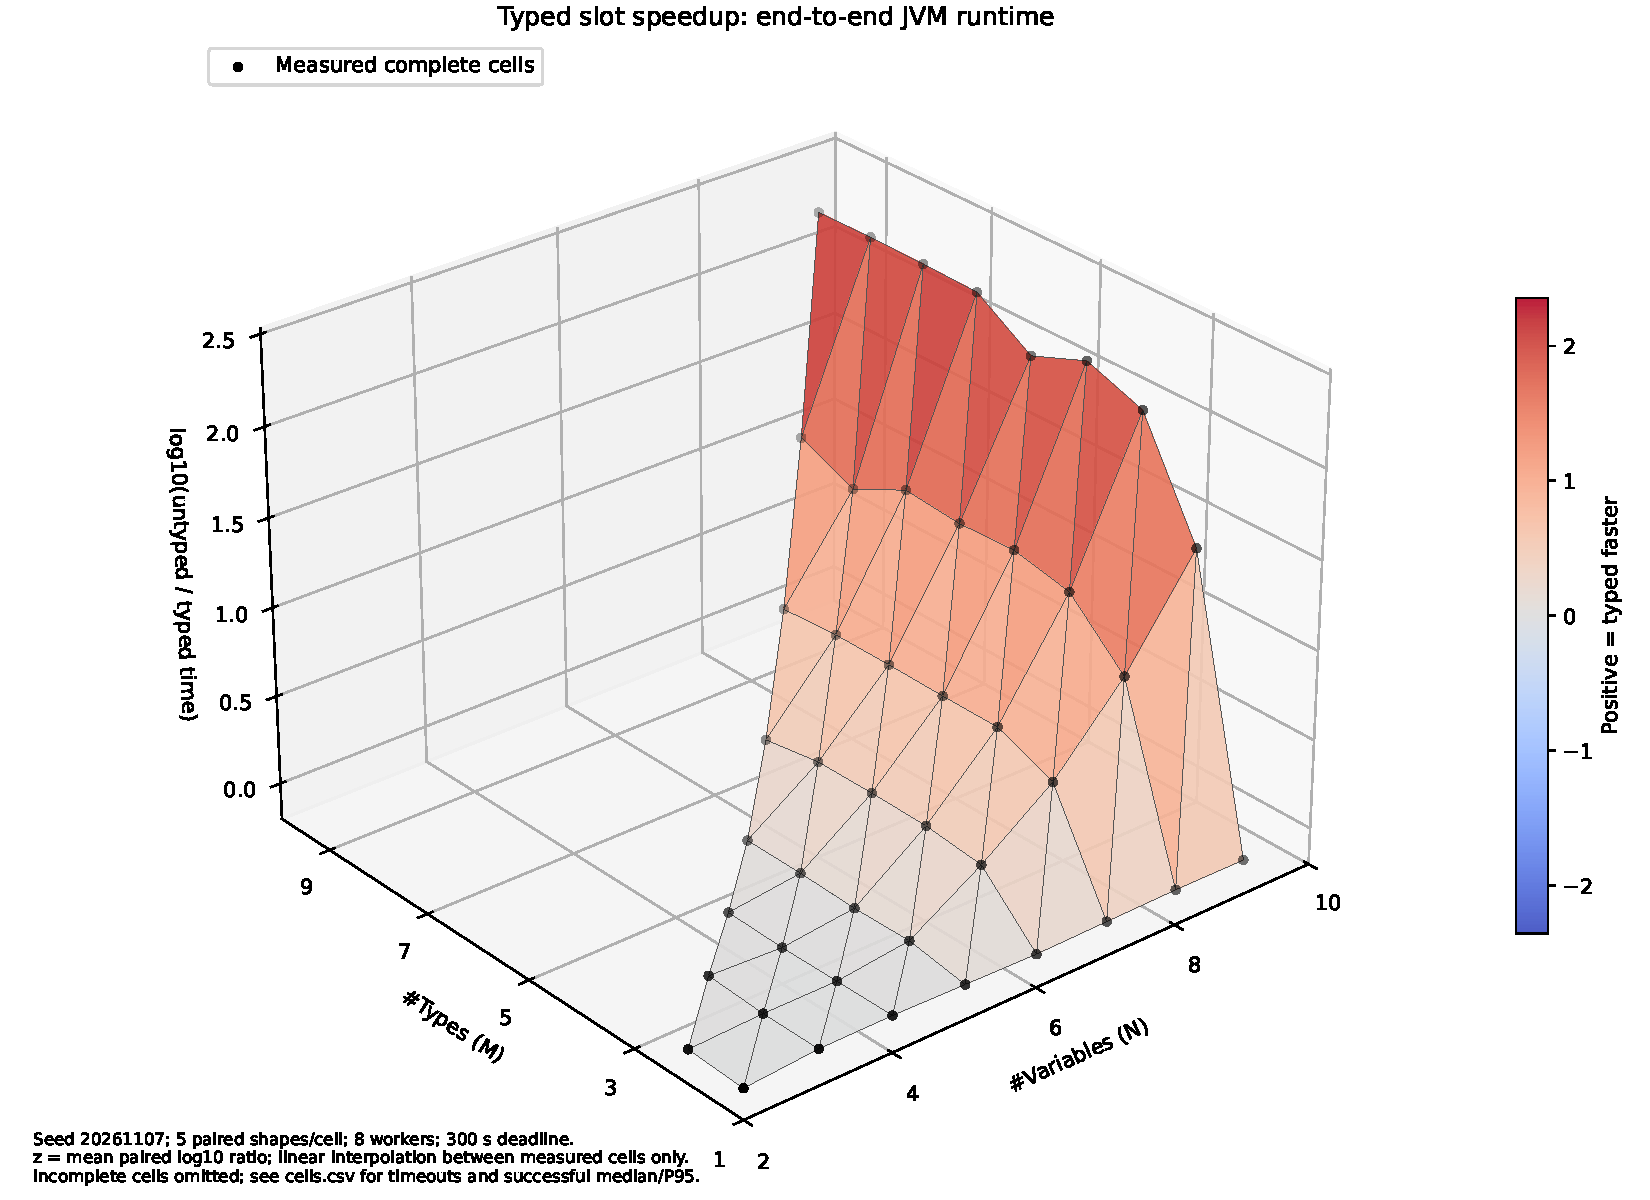
\includegraphics[width=0.78\linewidth]{figures/wall-speedup-surface.pdf}
\caption{Synthetic typed-versus-untyped end-to-end JVM speedup surface
($\log_{10}$ ratio across the 44/54 complete matched cells, without
interpolating across censored timeout cells). Complements
Figure~\ref{fig:synthetic-grid}.}
\label{fig:synthetic-wall-surface}
\end{figure}

\subsection{Bounded Semantic Validation Checks}

The natural checker evaluated 4,499 distinct zero
claims in the source models and found no counterexamples at the recorded
bounds. Each of the four deliberately invalid probes was refused by all
seven ablation arms. The capability study ran 29 bounded
sample checks across the generated families.

\subsection{Reproduction Identifiers}

\begingroup
\def\UrlBreaks{\do\-\do\_\do\/\do0\do1\do2\do3\do4\do5\do6\do7\do8\do9%
  \do\a\do\b\do\c\do\d\do\e\do\f}
\Urlmuskip=0mu plus 1mu\relax
The v3.3 experiment froze commit \path{d5c0c2a07504d53b13b28c61e9e64768c37eb984}.
It used 16 workers, an 8\,GiB heap cap, reward pool 100 and seed
\texttt{55520260811}. The following identifiers preserve the v3 synthetic
and historical study configuration.
\begin{itemize}
\item Experiment commit: \path{2d70f89ab67241cd071387ecedd3b2f432821921}.
\item Release commit (tag \texttt{v3}): \path{8770cb4b5f7133bad78058d9bc214f0ca36130d0}.
\item Natural corpus SHA-256 (66,080 files):
  \path{d6741fbf4c4a9b3714d012d068f84cc918052f1f55211bf4d0443b990736a689}.
\item Synthetic scaling dataset SHA-256 (270 pairs / 540 predicates):
  \path{c490b2bb1e6199f2ed221aa3f1b2d22b1da5dd8604341f305302c27a45de6b5f}.
\item Rule set: \texttt{canonical-equivalences-v3-explicit-laws};\\
  repair metric manifest ID:\\
  \texttt{certified-fast-rewrite-repair-distance-v25-}\\
  \texttt{retained-phase-representation}.
\item Natural and capability environment: AMD Ryzen~9 9950X3D (32 logical
  processors), OpenJDK~17.0.21.0.3, 16 workers, 8\,GiB heap, seed
  \texttt{55520260811}. Natural ablation run ID:
  \path{8dfc4fcc-84f0-4e9e-a88f-218fe05439b6}.
\item Synthetic grid environment: 8 concurrent isolated JVMs, 768\,MiB heap per
  JVM, 300-second deadline per predicate per arm; run ID:
  \path{e3d9bc4e-a514-471b-9e01-162562663f2e}.
\end{itemize}
\endgroup

\clearpage
\section{Rewrite Policy and Side Conditions}
\label{app:canon-rules}

Section~\ref{sec:canonicalization-procedure} describes canonical-record
construction. This appendix collects the rewrite choices used to expose and
normalize operands. A rule applies only to a typed operator instance whose side
conditions hold; the resulting source equation supplies the local certificate
consumed by the soundness argument.

\subsection{Rewrite Order and Side Conditions}
\label{app:rule-order}

The normalization order is parser cleanup, alpha normalization,
capture-avoiding let substitution, branch elimination, negation normalization,
phase-local prenexing and domain guarding, repeated negation and neutral
cleanup after unused-binding removal, membership elimination prior to
destructive distribution, container normalization, and local saturation with
rebuilding. Quantifier motion stays within a temporal phase unless an explicit
source law permits crossing its boundary.

Parser aliases share an internal head only when the frontend establishes the
same operator and type instance. Let substitution avoids capture via lifted de
Bruijn substitution, which preserves newly introduced bound positions while
substituting into outer scopes.

\paragraph{Boolean rules.}
Branch elimination uses
\begin{align*}
 A\Rightarrow B&=\neg A\lor B,\\
 A\Leftrightarrow B&=(\neg A\lor B)\land(\neg B\lor A),\\
 \operatorname{ite}(C,A,B)&=(C\land A)\lor(\neg C\land B)
\end{align*}
for formula-valued conditionals. Negation normalization applies double
negation, constant negation, and De Morgan's laws. Local saturation adds
Boolean identities, annihilators, idempotence, and complements:
\begin{align*}
 A\land\top&=A,& A\lor\bot&=A,&
 A\land\bot&=\bot,& A\lor\top&=\top,\\
 A\land A&=A,& A\lor A&=A,&
 A\land\neg A&=\bot,& A\lor\neg A&=\top.
\end{align*}
Recognizing complementary atoms requires equality of the underlying normalized
atoms, not merely matching operator names. Empty or singleton containers reduce
to units or children only when the operator's laws license those endpoints.

\paragraph{Temporal and atomic duals.}
Negation exchanges always/eventually, historically/once, until/releases, and
since/triggered with negated operands under the intended temporal semantics.
Atomic duals include equality/inequality, membership/nonmembership, and
complementary comparisons; unsupported operators keep an explicit negation.

\paragraph{Quantifiers, domains, and scheduling.}
Universal and existential negation swap the quantifier and negate the body,
while multiplicity quantifiers use their own duals (e.g., negating
\textsf{one} yields \textsf{notone}). Empty-domain laws handle each quantifier
explicitly: \textsf{all}, \textsf{no}, and \textsf{lone} over an empty domain
are true, whereas \textsf{some} and \textsf{one} are false. For finite
carriers $C$, predicates $p,d$, and $r$ independent of the bound variable,
\begin{align*}
 (\exists_C p)\land r&=\exists_C(\lambda x.\,p(x)\land r),&
 \exists_{\operatorname{filter}(d,C)}p&=\exists_C(\lambda x.\,d(x)\land p(x)),\\
 (\forall_C p)\lor r&=\forall_C(\lambda x.\,p(x)\lor r),&
 \forall_{\operatorname{filter}(d,C)}p&=\forall_C(\lambda x.\,\neg d(x)\lor p(x)).
\end{align*}
These identities hold even when $C$ is empty, whereas other quantifier/connective
combinations may require nonemptiness and are not generalized by analogy.
Unused-binder removal is followed by neutral cleanup so equivalent subterms
reached by different simplification paths stabilize to the same shape, and
membership elimination on relations runs before destructive distribution so
source shapes needed by guarded rewrites are preserved.

Binder-block permutations must preserve the full descriptor—types, domains,
multiplicities, disjointness classes, and dependencies—rather than merely
permuting slots of matching types.

\subsection{Operator Profiles}

The Alloy operator profile assigns carriers as follows:
\begin{itemize}
\item Boolean conjunction and disjunction, and relational union and
  intersection, use $\Set$ ports with licensed flattening.
\item Integer addition and multiplication use $\Bag$ ports; flattening is
  licensed for modular $\operatorname{Fin}(2^w)$ arithmetic, whereas with
  overflow rejection $(7+1)+(-1)$ fails in signed 4-bit arithmetic while
  $7+(1+(-1))=7$, forbidding unguarded reassociation.
\item Equality, inequality, and biconditional use commutative binary ports
  without recursive flattening.
\item Relational join, product, calls, and total-order predicates retain
  positional ports; disjointness predicates use nonflat bags.
\end{itemize}
Under Alloy's subset semantics, $x\ \texttt{in}\ \texttt{none}$ reduces to false
only when $x$ is known nonempty, since an empty relation is a subset of
\texttt{none}. Finally, canonical equality ($d=0$ under a complete finite
presentation) tests membership in the declared structural quotient, whereas
repair distance ($d_{\mathrm{repair}}>0$) measures structural edits between
repair projections; Section~\ref{sec:evaluation} reports them separately.

\fi
\end{document}
